\documentclass[12pt,a4paper]{article}
\usepackage[utf8]{inputenc}
\usepackage[czech, english]{babel}
\usepackage[T1]{fontenc}
\usepackage{amsmath}
\usepackage{amsfonts}
\usepackage{amssymb}
\usepackage{graphicx}
\usepackage[final,pdftex, colorlinks=false]{hyperref}
\usepackage{xcolor}
\usepackage{comment}
\usepackage{todonotes}
\usepackage{floatrow}
\usepackage{multirow}
\usepackage{algorithm}
\usepackage{algorithmicx}
\usepackage{algpseudocode}
\usepackage{titletoc}
\usepackage{pdfpages}
\usepackage{hhline}
\usepackage{makecell}

\usepackage{listings}			%vkladani kodu
\lstset{basicstyle=\ttfamily,
  showstringspaces=false,
  commentstyle=\color{red},
  keywordstyle=\color{blue},
  breaklines=true,
  frame=lines,
}

%okraje
\usepackage[
left=35mm,
right=25mm,
top=40mm,
bottom=35mm]
{geometry}

\author{Adam Laža}

%%%%%%%%%%Prikazy%%%%%%%%%%
\renewcommand\baselinestretch{1.3}		%radkovani
\parskip=0.8ex plus 0.4ex minus 0.1 ex	%mezera mezi odstavci

\newcommand{\keywords}[2]{\noindent\textbf{#1: }#2}
\newcommand{\necislovana}[1]{%
\phantomsection
\addcontentsline{toc}{section}{#1}

%\newcommand{\exedout}{%
%  \rule{0.8\textwidth}{0.5\textwidth}%
%}


\section*{#1}
\markboth{\uppercase{#1}}{}
}
%%%%%%%%%%%%%%%%%%%%%%%%%%%%

%%%%%%%%%%Zahlavi%%%%%%%%%%%
\usepackage{fancyhdr}
\fancyhead[L]{CTU in~Prague}
\setlength{\headheight}{16pt}
%%%%%%%%%%%%%%%%%%%%%%%%%%%%

\begin{document}
\pagestyle{empty}

\newpage
\begin{center}
%napisy
\newcommand{\napisCVUT}{Czech technical university in Prague}
\newcommand{\napisFS}{Faculty of Civil engineering}
\newcommand{\napisProgram}{Study programme Geodesy and cartography}
\newcommand{\napisObor}{Geomatics}
\newcommand{\napisKatedra}{Department of geomatics}
\newcommand{\napisVedouci}{Supervisor: Ing. Martin Landa, Ph.D.}
\newcommand{\napisAutor}{Bc. Adam Laža}
\newcommand{\napisDatum}{Prague 2018}
\newcommand{\napisNazevI}{Process isolation in PyWPS framework}
\newcommand{\napisNazevAjI}{Izolace procesů ve frameworku PyWPS}
\newcommand{\napisDiplomka}{Master thesis}
\newcommand{\napisPraha}{Prague 2018}
%
% prikazy
%\newcommand{\velka}[1]{\uppercase{#1}}
\newcommand{\velka}[1]{\textsc{#1}}
%
% 
\newif\ifpatitul
\patitultrue

\ifpatitul
{\Large\velka{\napisCVUT}}\\
\velka{\Large\napisFS}\\
\vfill
{\LARGE\velka{\napisDiplomka}}
\vfill
{\large\napisPraha\hfill\napisAutor}
\newpage
\fi%patitul


{\Large\velka{\napisCVUT}}\\
{\Large\velka{\napisFS}}\\
{\Large\velka{\napisProgram}}\\
{\Large\velka{\napisObor}}
\vfill

\includegraphics[width=3cm]{logo_cvut_cb} %~
\vfill
{\Large\velka{\napisDiplomka}}\\
\Large\velka{\napisNazevI}\\
\large\velka{\napisNazevAjI}
\vfill
{\large%
\napisVedouci\\
\napisKatedra\\
\bigskip
\napisDatum\hfill\napisAutor}
\end{center}


\newpage
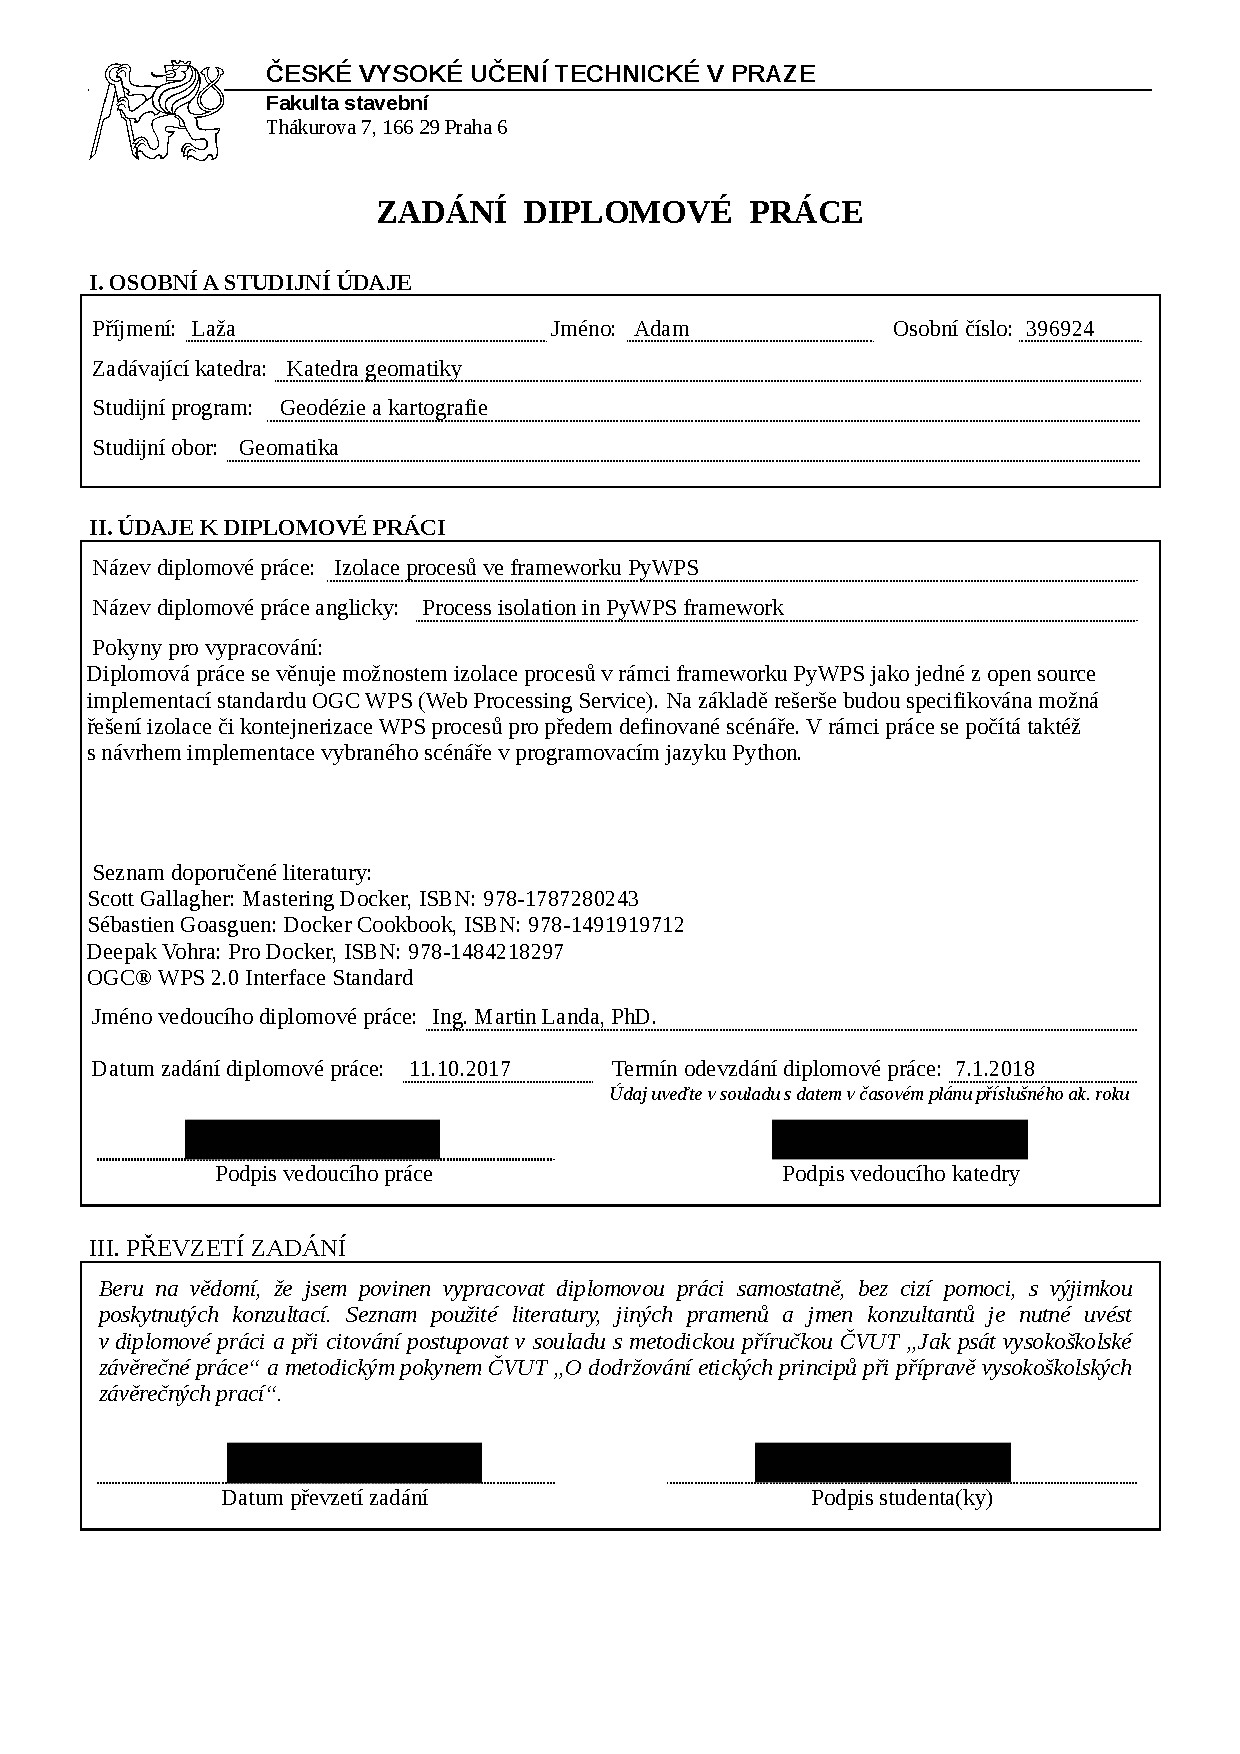
\includepdf[pages={1}]{../zadani/zadanidp.pdf}

\newpage

\selectlanguage{english}
\begin{abstract}
\bigskip
This master thesis is dedicated to a process isolation in PyWPS framework as one of the OGC WPS implementation. OGC WPS is Web Processing Service
Standard defined by Open Geospatial Consortium.

The first part describes the standard itself including all three mandatory operations
\textit{GetCapabilities}, \textit{DescribeProcess} and \textit{Execute}. At the end of the first part some implementations of the standard
are mentioned.

The second part concentrates on \textit{PyWPS}, one of the WPS implementation written in Python. Readers are introduced to the current
state of PyWPS as well as to \textit{PyWPS-demo} project, a demo server isntance, which the implementation part is based on. A research about possible solutions of process isolation follows and then \textit{Docker} technology is described as final choice for implementaion.

The third part covers the implementation of Docker containers for process isolation. The workflow of \textit{Execute} operation is
described in detail and brand new \textit{Container} class with all its methods is introduced.

\bigskip
\bigskip
\keywords{Keywords}
OGC WPS, PyWPS, Docker container, Python, process isolation, Web Processing Service, geoprocessing.
\end{abstract}

\newpage
\selectlanguage{czech}
\begin{abstract}
\bigskip
Tato diplomová práce se věnuje možnostem izolace procesů v rámci frameworku PyWPS jako jedné z implementací OGC WPS. Web Processing 
Service je standard vydaný a dále rozšiřovaný Open Geospatial Consorciem. 

První část popisuje samotný standard včetně všech základních požadavků \textit{GetCapabilities}, \textit{DescribeProcess} a \textit{Execute}.
V závěru první části jsou zmíněny některé z implementací WPS standardu.

Druhý část se zaměřuje na \textit{PyWPS}, což je implementace WPS standardu napsaná v programovacím jazyce Python. Čtenáři jsou seznámeni
jak se současným stavem PyWPS, tak s projektem \textit{PyWPS-demo}, ukázkovou instancí PyWPS serveru, na kterém je postavena praktická část. 
Následuje rešerše, která mapuje možné řešení izolace procesů, a nakonec je popsána \textit{Docker} technologie, která slouží pro kontejnerizaci
a která byla vybrána pro samotnou implementaci izolace.

Poslední část se zabývá použitím Docker kontejnerů pro izolaci procesů. Detailně je vysvětleno, jak funguje \textit{Execute} operace a následně je popsána nově vytvořená třída \textit{Container} se všemi svými metodami.

\bigskip
\bigskip
\keywords{Klíčová slova}
OGC WPS, PyWPS, Docker kontejner, Python, izolace procesu, geoprocesing, zpracování dat.
\end{abstract}

\selectlanguage{english}
%%%%Prohlaseni a podekovani
\newcommand{\odsaditodzhora}{\hskip1pt\vfill}
\newpage
\odsaditodzhora
\noindent {\bf Declaration of authorship}
I declare that the work presented here is, to the best of my knowledge and
belief, original and the result of my own investigations, except as acknowledged.
Formulations and ideas taken from other sources are cited as such.


\begin{flushleft}
\begin{tabular}{cp{0.3\textwidth}c}
In Prague .................
& 
&
..................................
\\
&&
(author sign)
\end{tabular}

\end{flushleft}
\newpage

\odsaditodzhora
\noindent {\bf Acknowledgement}

\todo[inline]{Podekovani}

\newpage
\tableofcontents

\newpage
\pagestyle{fancy}

\necislovana{Introduction} 
There are data all around us. As the society is becoming more and more digitalized the amount of the data is getting
bigger and bigger. A lot of enterprises, institutions and organizations realize that these data hide a huge potential
they can profit from. However the data themselves in their raw form are not usually sufficient to make a
conclusion from them. More often the data need to be processed and used as an inputs data for some kind of analyses. 
With the increasing number of gathered data a manual processing is almost inconceivable. Data are processed in an automatized way. 

Therefore, in order to be able to process the data independently of the type of acquisition, format or platform, 
it is necessary to define standards. Regarding spatial data, these standards are made by the Open Geospatial Consortium. 
Besides quite famous and used standards as WMS and WFS there also exists the WPS standard. The WPS standard defines an 
interface that facilitates the publishing of geospatial processes. It also provides rules how inputs and outputs are handled.
The WPS is only a standard and there are several implementations. This work is primarily focused on the \textit{PyWPS} framework.

\bigskip
The main topic of this thesis is process isolation. A process is just some geospatial operation which has its defined
inputs and outputs and which is deployed on a server. The server is able to execute multiple 
processes at the same time. This thesis deals with the isolation of individual processes especially for security and 
performance reasons. With every process fully isolated so they cannot interact with each other the higher security level
is assured.

The thesis is composed of several parts. The introductory research discusses the current state of the PyWPS and the
other projects that implement the WPS standard, namely \textit{ZOO-Project} and \textit{52$^{\circ}$North}. Then the
introducing research offers possible solutions to achieve process isolation. Various projects and technologies are
described and finally the Docker has been selected as the technology we try to implement in the practical part. Docker
has been selected as one of the most used technology for containerization. It puts every process into a separate
container so the isolation is ensured. Moreover Docker provides a mechanism to pause, stop and start a container so it
looks like a possible solution for the future WPS 2.0.0 standard implementation which requires this functionality. Using
Docker it also opens new possibilities, e. g. being able to deploy running job to cloud.

The technological background is covered in the second part. There is the WPS standard described, especially its operations
- \textit{GetCapabilities}, \textit{DesribeProcess} and \textit{Execute} - and inputs and outputs structures. There are also
\textit{PyPWS} and \textit{Docker} described.

Last part consists of the implementation description.
\todo[inline]{Doplnit uvod o implementaci}

I have chosen this topic to get in touch with another OGC standard. I also appreciate I can dive more into Docker technology
as it is a leader in containerization in the world.

\newpage
\part{Web Processing Service}
\newpage
\section{Web Processing Service}

\subsection{History}
The first mention of the Web Processing Service was in October 2004. Back then it
was named Geoprocessing Service \cite{OGC_news}. The specification was first 
implemented as a prototype in 2004 by Agriculture and Agri-Food Canada (AAFC).
In its further development during a Geoprocessing Services Interoperability Experiment \cite{WPS_experiment} 
the name was changed to "Web Processing Service" to avoid the acronym GPS, since 
this would have caused confusion with the conventional use of this acronym for 
Global Positioning System \cite{WPS_standart_1.0}. The first version of WPS was released in
September 2005 \cite{WPS_first}. The experiment demonstrated that various clients
could easily access and bind to services which were set up according to the WPS Implementation
specification.

Currently two major versions of WPS Standard exist. The WPS version 1.0.0 is currently used mostly.
If not explicitly said this thesis is dedicated to the version 1.0.0. The WPS version 2.0.0 was
released in 2015 \cite{WPS_second}.

\subsection{Open Geospatial Consortium}
The OGC \textit{Open Geospatial Consortium} is an international non-profit organization committed to making quality 
open standards for the global geospatial community. These standards are made through a consensus process and are freely available for anyone to use to improve sharing of the world's geospatial data. The OGC members come from government, commercial organizations, NGOs, academic and research organizations.\cite{OGC}

A predecessor organization, OGF, the Open GRASS Foundation, started in 1992. From 1994 the organization 
used the name \textit{Open GIS Consortium}, in 2004 the Board changed the name to \textit{Open Geospatial Consortium}.\cite{OGC_history}

Some of the widely-use OGC standards are:
\begin{itemize}
\item WCS, WMS, WFS, WMTS or WPS - standards for web services
\item GML, KML - standards for XML-based languages
\end{itemize}


\bigskip
\subsection{Web Processing Service}
The OGC Web Processing Service (WPS) Interface Standard defines a standardized interface
that facilitates the publishing of geospatial processes. Also provides rules how to standardize
requests and responses for geospatial processing services. 

\textit{Process} means any operation on spatial
%% ML: as -> like ?
%% AL: opraveno
data from simple ones like maps overlay or buffering to highly complex as complicated global models. Any kind of GIS 
functionality can be offered to clients across a network with correctly configured WPS. 

\textit{Publishing} means
creating human-readable metadata that allow users to discover and use service as well as making 
available machine-readable binding information.

\textit{Data} can be both vector or raster data and can be delivered across the network or be available
at the server.

The interface does not specify any specific processes that can be implemented by a WPS nor any specific
data inputs or outputs. Instead it specifies generic mechanisms to describe any geospatial process and
data required and produced by the process. The interface does not only provide mechanisms for calculation
but also to identify required data, initiate the calculation and manage output data so clients can access it. 

\bigskip
Web Processing Service as one of the OGC web services specifies three types of requests which can be requested
by a client and performed by a WPS server. The implementation of these three requests is mandatory by all servers:

\textbf{\textit{GetCapabilities}} - The request returns to the client a Capabilities document that describes the abilities
of the specific server implementation. It also returns the name and abstract of each of the processes that can
be run on a WPS instance.

\textbf{\textit{DescribeProcess}} - The request returns details about the processes offered by a WPS instance. Describes
required inputs and produced outputs and their allowable formats.

\textbf{\textit{Execute}} - The request allows the client to run a specified process with provided parameters and returns
produced outputs.

\newpage
These operations are very similar to other OGC Web Services such as WMS, WFS, and WCS. Common interface aspects
are defined in the OGC Web Services Common Implementation Specification \cite{OGC_common}. As seen in 
the class diagram at Fig. \ref{fig:WPS_class_diagram} the~WPS interface class inherits the GetCapabilities operation 
from OGCWebService interface class. The operations Execute and DescribeProcess are specific for the WPS. The WPS
%% ML: vysvetlit v poznamce pod carou co je get a post?
%% AL: vysvetleno.
operations are based on HTTP GET\footnote{\textit{HTTP GET} requests data from a specified resource. Data are sent in the URL of a GET request.} and 
POST\footnote{\textit{HTTP POST} submits data to be processed to a specified resource. Data are sent inside the HTTP message body of
POST request} requests.

\begin{figure}[h!]
\centering
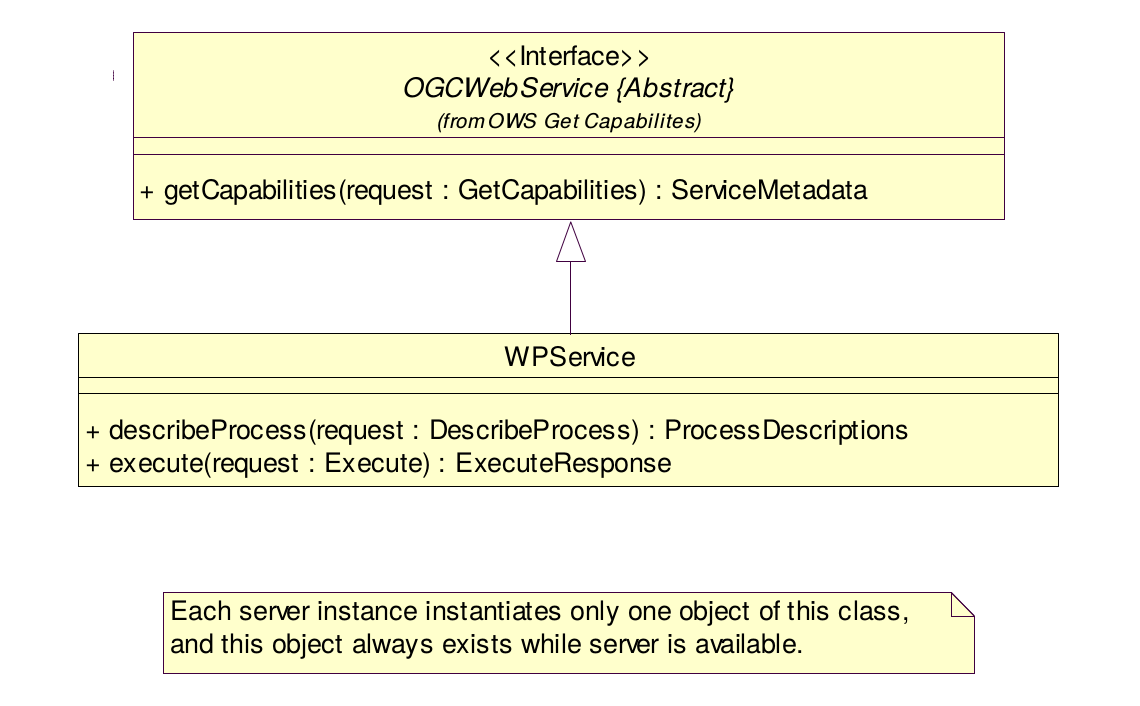
\includegraphics[width=0.78\textwidth]{img/WPS_class_diagram.png}
\caption{WPS interface UML description, source: \cite{WPS_standart_1.0}}
\label{fig:WPS_class_diagram}
\end{figure}

%% ML: mas nekde vystetleno co je KVP a XML encoding?
%% AL: vysvetleno.
The GetCapabilities and DescribeProcess shall use HTTP GET with KVP encoding and Execute operation shall use HTTP
POST with XML encoding. Summarized in Tab. \ref{tab:WPS_encoding}.
\begin{table}[h!]
\catcode`\-=12
\centering
\begin{tabular}{|c|c|c|}
\hline
%% ML: proc je hlavicka mensim pismem?
%% AL: mne se hlavicka vykresluje stejne velkym pismem.
\multirow{2}{*}{Operation} & \multicolumn{2}{c|}{Request encoding} \\ \cline{2-3} 
                           & Mandatory          & Optional         \\ \hhline{|=|=|=|}
GetCapabilities            & KVP                & XML              \\ \hline
DescribeProcess            & KVP                & XML              \\ \hline
Execute                    & XML                & KVP              \\ \hline
\end{tabular}
\caption{Operations request encoding}
\label{tab:WPS_encoding}
\end{table}


\paragraph{KVP encoding} are key-value pairs usually sent via HTTP GET request method encoded directly in the URL. The 
keys and values are separated with = sign and each pair is separated with \& sign  or with ? sign at the beginning of 
the request. Example could be the get capabilities request:

\begin{lstlisting}[basicstyle=\small,caption={GetCapabilities with KVP encoding.}]
http://server.domain/wps?service=WPS&request=GetCapabilities&version=1.0.0
\end{lstlisting}

In this example, there are 3 pairs of input parameter: service, request and version with values WPS, GetCapabilities and 
1.0.0 respectively.\cite{PyWPS_docs}

\paragraph{XML payload} is XML data sent via HTTP POST request method. The XML document can be more rich, having more 
parameters, better to be parsed in complex structures. The Client can also encode entire datasets to the request, 
including raster (encoded using base64) or vector data (usually as GML file).\cite{PyWPS_docs}

\begin{lstlisting}[basicstyle=\small,caption={GetCapabilities XML payload example}]
<?xml version="1.0" encoding="UTF-8"?>
<wps:GetCapabilities language="cz" service="WPS" xmlns:ows="http://www.opengis.net/ows/1.1" xmlns:wps="http://www.opengis.net/wps/1.0.0" xmlns:xsi="http://www.w3.org/2001/XMLSchema-instance" xsi:schemaLocation="http://www.opengis.net/wps/1.0.0 http://schemas.opengis.net/wps/1.0.0/wpsGetCapabilities_request.xsd">
  <wps:AcceptVersions>
    <ows:Version>1.0.0</ows:Version>
  </wps:AcceptVersions>
</wps:GetCapabilities>
\end{lstlisting}

\subsubsection{GetCapabilities}
The GetCapabilities operation is mandatory. The operation allows a client to retrieve capabilities document (metadata)
from a server. The response XML document contains service metadata about the server and all implemented processes description.

\paragraph{GetCapabilities request}

\begin{table}[h!]
\catcode`\-=12
\centering
\begin{tabular}{|c|c|c|}
\hline
\thead{Name}               & \thead{Optionality and use} & \thead{Definition and format}    		\\ \hhline{|=|=|=|}
service=WPS                & Mandatory           & Service type identifier text 	\\ \hline
request=GetCapabilities    & Mandatory           & Operation name text              \\ \hline
AcceptVersion=1.0.0        & Optional            & Specification version            \\ \hline
Sections=All               & Optional            & \makecell{Comma-separated \\unordered list of sections} \\ \hline
updateSequence=XXX         & Optional            & \makecell{Service metadata \\document version}            \\ \hline
AcceptFormats=text/xml     & Optional            & \makecell{Comma-separated prioritized \\sequence of response formats} \\ \hline
\end{tabular}
\caption{GetCapabilities operation request URL parameters, source: \cite{OGC_common}}
\label{tab:WPS_GetCapabilities}
\end{table}

\begin{itemize}
\item\textit{service} - A mandatory parameter, WPS is only possible value.
\item\textit{request} - A mandatory parameter, GetCapabilities is only possible value.
\item\textit{version} - An optional parameter, version number. Three non-negative integers separated by a decimal point. Servers and
their clients should support at least one defined version.
\item\textit{sections} - An optional parameter that contains a list of section names. Possible values are: \textit{ServiceIdentification,
ServiceProvider, OperationsMetadata, Contents, All}.
\item\textit{updateSequence} - An optional parameter for maintaining the consistency of a~client cache of the contents of a service
metadata document. The parameter value can be an integer, a timestamp, or any other number or string.
\item\textit{format} - An optional parameter that defines response format.
\end{itemize}

A client can request the GetCapabilities operation with parameters from the Tab. \ref{tab:WPS_GetCapabilities}. A corresponding
request URL looks like:

\noindent
\url{http://localhost:5000/wps?service=WPS&request=GetCapabilities&AcceptVe}\\
\url{rsion=1.0.0&Section=ServiceIdentification,OperationsMetadata&updateSeq}\\
\url{uence=XXX&AcceptFormats=text/xml}

\paragraph{GetCapabilities response}
\label{para:GetCapa_response}
%% ML: co znamena Normal?
%% AL: jakoze neskonci s exception. Ale mozna je ten nadpis matouc, mazu
When GetCapabilities operation is requested a client retrieve service metadata document that contains sections specified in
\textit{sections} parameter. If the parameter value is \textit{All} or not specified than all sections are retrieved.

\begin{itemize}
\item\textit{ServiceIdentification} - Server metadata.
\item\textit{ServiceProvider} - Server operating organization metadata.
\item\textit{OperationsMetadata} - Metadata about operations implemented by the WPS server, including URLs to request them.
\item\textit{ProcessOfferings} - List of processes with name and brief description implemented by the WPS server.
\end{itemize}

\bigskip
In addition to sections each GetCapabilities response should contain:
\begin{itemize}
\item\textit{version} - Specification version for GetCapabilities operation.
\item\textit{updateSequence} - Server metadata document version, value is increased whenever any change is made in complete service metadata document.
\end{itemize}

\subparagraph{GetCapabilities exceptions}
In case that WPS server encounters an error a~client retrieves an exception report message with one of the exception code:

\begin{itemize}
\item\textit{MissingParameterValue} - GetCapabilities request does not contain a required parameter value.
\item\textit{InvalidParameterValue} - GetCapabilities request contains an invalid parameter value.
\item\textit{VersionNegotiation} - Any version from AcceptVersions parameter list does not match any version supported by the WPS server.
\item\textit{InvalidUpdateSequence} - Value of updateSequence parameter is greater than current value of service metadata updateSequence number.
\item\textit{NoApplicableCode} - Other exceptions.
\end{itemize}

\subsubsection{DescribeProcess}
The DescribeProcess operation is mandatory. The operation allows clients to retrieve a detailed description of one or more
processes implemented by a WPS server. The detailed information describes both required inputs and produced outputs and allowed
formats.

\begin{table}[h!]
\catcode`\-=12
\centering
\begin{tabular}{|c|c|c|}
\hline
\thead{Name}               & \thead{Optionality} & \thead{Definition and format}    		\\ \hhline{|=|=|=|}
service=WPS                & Mandatory           & Service type identifier text 	\\ \hline
request=DescribeProcess    & Mandatory           & Operation name text              \\ \hline
version=1.0.0              & Mandatory           & WPS specification version            \\ \hline
Identifier=buffer          & Optional            & \makecell{List of one or more process\\ identifiers, separated by commas} \\ \hline
\end{tabular}
\caption{DescribeProcess operation request URL parameters, source: \cite{OGC_common}}
\label{tab:WPS_DescribeProcess}
\end{table}

\paragraph{DescribeProcess request}
\begin{itemize}
\item\textit{service} - Mandatory parameter, WPS is only possible value.
\item\textit{request} - Mandatory parameter, DescribeProcess is only possible value.
\item\textit{version} - Mandatory parameter, version number. Three non-negative integers separated by decimal point. Servers and
their clients should support at least one defined version.
\item\textit{Identifier} - Optional parameter, list of process names separated by comma. Another possible value is \textit{all}.
\end{itemize}

The DescribeProcess operation can be requested with parameters from Tab. \ref{tab:WPS_DescribeProcess}. A corresponding
request URL looks like: \url{http://localhost:5000/wps?request=DescribeProcess&service=WPS&identifier=all&version=1.0.0}

\paragraph{DescribeProcess response}
\label{para:DesribeProc_response}

%% ML: Normal? viz poznamka vyse
%% AL: Smazano
A response to DescribeProcess request contains one or more process descriptions for requested process identifiers.
%% ML: co to je za strukturu, zde poprve pouzivas kurzivu, z toho mam pocit, ze jde o neco podstatneho ;-)
%% ML: nikde jinde o strukture nemluvis, to je matouci
%% AL: prepsal jsem odstavec, snad je to srozumitelnejsi
Each
process description contains detailed information about process in ProcessDescription XML element (see Tab. 
\ref{tab:WPS_ProcessDescription})
including process inputs and outputs description. The number of inputs or outputs is not limited.

\bigskip
\begin{table}[h!]
\catcode`\-=12
\centering
\begin{tabular}{|c|c|c|}
\hline
\thead{Name}               & \thead{Optionality} & \thead{Definition and format}    		\\ \hhline{|=|=|=|}
Identifier      	       & Mandatory           & Process identifier             \\ \hline
Title 			           & Mandatory           & Process title 				  \\ \hline
Abstract		           & Optional            & Brief description              \\ \hline
Metadata		           & Optional            & \makecell{Reference to more metadata about this process} \\ \hline
Profile			           & Optional            & \makecell{Profile to which the WPS process complies} \\ \hline
processVersion	           & Mandatory           & Release version of process \\ \hline
WSDL    		           & Optional            & \makecell{Location of a WSDL document that \\describes this process} \\ \hline
DataInputs		           & Optional            & \makecell{List of the required and optional inputs} \\ \hline
ProcessOutputs	           & Mandatory           & \makecell{List of the required and optional outputs} \\ \hline
storeSupported	           & Optional            & \makecell{Complex data outputs can be \\stored by WPS server} \\ \hline
statusSupported	           & Optional            & \makecell{Execute response can be returned\\ quickly with status information} \\ \hline
\end{tabular}
\caption{Parts of ProcessDescription data structure, source: \cite{WPS_standart_1.0}}
\label{tab:WPS_ProcessDescription}
\end{table}

\noindent
Three data types of input or outputs exist:
\begin{itemize}
\item\textit{LiteralData} - any string. It is used for passing single parameters like numbers or text parameters. There can be set
\textit{allowedValues} restriction. It can be a~list of allowed values or input data type. Additional attributes such as \textit{units}
or \textit{encoding} can be set as well. 
\item\textit{ComplexData} - Complex data can be raster, vector or any file-based data, which are usually processed. ComplexData
%% ML: vysvetlit mimeType, poznamka pod carou?
%% AL: vysvetleno
are often result of the process. The input can be specified more using 
mimeType\footnote{\textit{mimeType} - is a standardized way to indicate the nature and format of a document. Browsers often use the MIME type (and not the file extension) to determine how it will process a document.}, XML schema or encoding.
\item\textit{BoundingBoxData} - BoundingBox data are specified in OGC OWS Common specification as two pairs of 
coordinates (for 2D and 3D space). They can either be encoded in WGS84 or EPSG code can be passed too. They are intended 
to be used as definition of the target region.
\end{itemize}

\subparagraph{DescribeProcess exceptions}
In case that WPS server encounters an error a~client retrieves an exception report message with one of the exception code:
\begin{itemize}
\item\textit{MissingParameterValue} - GetCapabilities request does not contain a required parameter value.
\item\textit{InvalidParameterValue} - GetCapabilities request contains an invalid parameter value.
\item\textit{NoApplicableCode} - Other exceptions.
\end{itemize}

\subsubsection{Execute}
The Execute operation is mandatory. The operation allows clients to run a specified process implemented by a server.
Inputs can be included directly in the request body or be referenced as a web-accessible resource. The outputs are 
returned in XML response document, either directly embedded within the response document or stored as a resource 
accessible by returned URL.

\bigskip
\begin{table}[h!]
\catcode`\-=12
\centering
\begin{tabular}{|c|c|c|}
\hline
\thead{Name}               & \thead{Optionality} & \thead{Definition and format}    		\\ \hhline{|=|=|=|}
service          	       & Mandatory           & Service type identifier text             \\ \hline
request			           & Mandatory           & Operation name text 				  \\ \hline
version			           & Mandatory           & WPS specification version              \\ \hline
Identifier   	           & Mandatory           & Process identifier \\ \hline
DataInputs		           & Optional            & \makecell{List of inputs provided \\ to this process execution} \\ \hline
ResponseForm	           & Optional            & Response type definition \\ \hline
language   		           & Optional            & Language identifier \\ \hline
\end{tabular}
\caption{Parts of Execute operation request, source: \cite{WPS_standart_1.0}}
\label{tab:WPS_ExecuteRequest}
\end{table}

%% ML: OK, tady uz zadne Normal neni... :-)
\paragraph{Execute request}
%% ML: Zkus odstavec prepsat, je to utrzkovite...
%% AL: trochu prehazena struktura a prepsany text
Execute request is usually sent via HTTP POST request. It triggers an execution of a specified process if no exceptions
raised (for instance ServerBusy). Execute request contains parameters from Tab. \ref{tab:WPS_ExecuteRequest}. Example of 
Execute XML response document sent within the POST request can be found at App. \ref{app:ExecuteRequest}. 


\paragraph{Execute response}
Usually the Execute operation response document is an XML document. The only exception is in case when a response form
of \textit{RawDataOutput} is requested, execution is successful and only one complex output is created, then directly
the produced complex output is returned. The result can be inserted directly inline the response document or be
referenced as web-accessible resource, it depends on ResponseForm request elements.

\begin{figure}[h!]
\centering
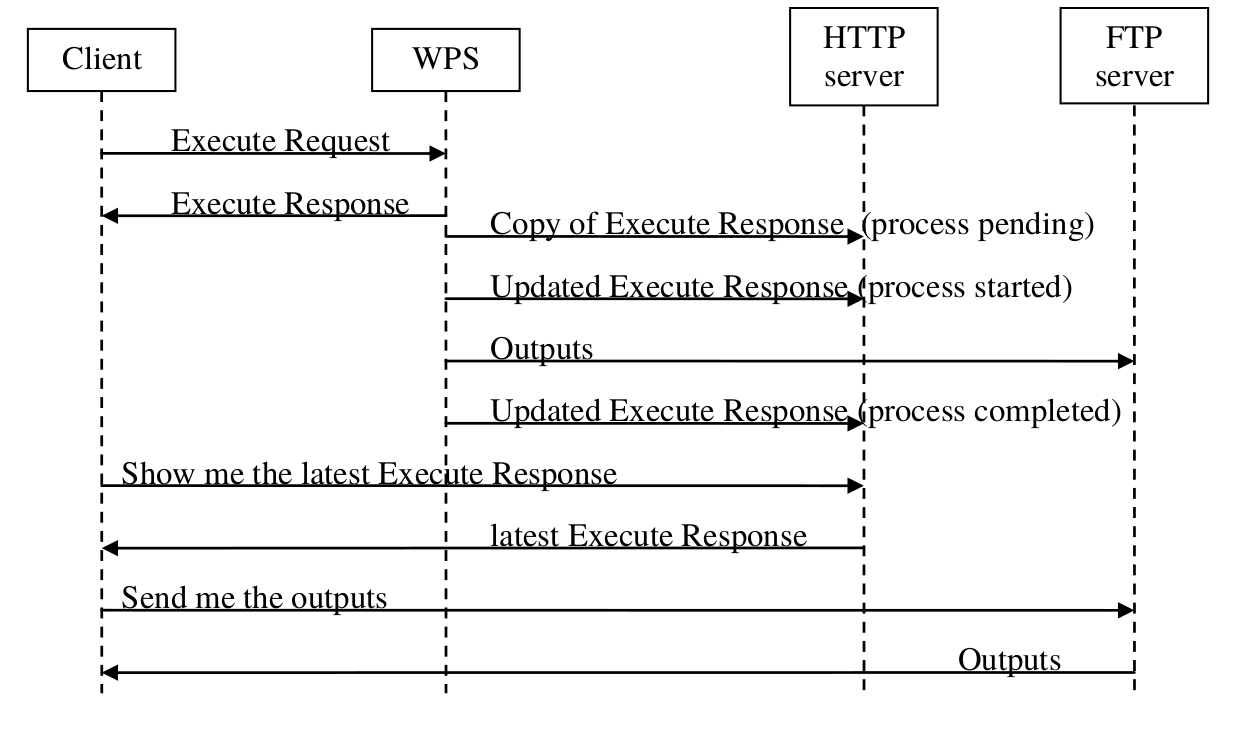
\includegraphics[width=0.8\textwidth]{img/WPS_sequence.png}
\caption{Sequence diagram: a client requests storage of results, source: \cite{WPS_standart_1.0}}
\label{fig:WPS_sequence}
\end{figure}

%% ML: right after hned ve dvou vetach po sobe...
%% AL: opraveno
In synchronous mode the response document is returned when the process execution is completed. However in asynchronous
mode it is possible to get
response document right after sending a request. In this case, returned response document contains a URL link from which 
the final response document can be retrieved after completed process execution. A~client can request execution status 
update to find out the amount of processing remaining if the execution is not completed. Shown in Fig. 
\ref{fig:WPS_sequence}.

%% ML: Podobna veta je na zacatku predesleho odstavce
%% AL: Prepsano.


\newpage
\begin{table}[h!]
\catcode`\-=12
\centering
\begin{tabular}{|c|c|c|}
\hline
\thead{Name}               & \thead{Optionality} & \thead{Definition and format}    		\\ \hhline{|=|=|=|}
service          	       & Mandatory           & Service type identifier text             \\ \hline
version			           & Mandatory           & WPS specification version              \\ \hline
language   		           & Mandatory           & Language identifier \\ \hline
statusLocation	           & Optional            & \makecell{Reference to location where current\\ExecuteResponse document is stored} \\ \hline
serviceInstance	           & Mandatory           & \makecell{Reference to location where current\\ExecuteResponse document is stored} \\ \hline
Process			           & Mandatory           & Process description \\ \hline
Status			           & Mandatory           & Execution status of the process \\ \hline
DataInputs		           & Optional            & \makecell{List of inputs provided \\ to this process execution} \\ \hline
OutputDefinitions          & Optional            & \makecell{List of definitions of outputs \\desired from executing this process} \\ \hline
ProcessOutputs             & Optional            & \makecell{List of values of outputs \\ from process execution} \\ \hline
\end{tabular}
\caption{Parts of ExecuteResponse data structure, source: \cite{WPS_standart_1.0}}
\label{tab:WPS_ExecuteResponse}
\end{table}

\newpage
\section{WPS implementations}
The OGC WPS is just an interface standard that provides rules for
%% ML: requests (mnozne cislo), response (jednotne) - je v tom nejaky zamer?
%% AL: opraveno
standardizing requests and responses. It also defines how clients can
request the execution of defined processes and how the outputs are
handled. There are several projects that implement this standard
across the platforms or programming languages.

\subsection{deegree}

%% ML: their zni v odstavci divne
%% AL: opraveno
\textit{deegree} is open-source community-driven project for spatial
data infrastructure written in Java. Besides from the other OGC Web
Services it implements also WPS standard 1.0.0. The implementation offers
sending request with KVP, XML or SOAP encoding,
asynchronous/synchronous execution and API for implementing processes
in Java. On their website there is a WPS demo
\footnote{\url{http://demo.deegree.org/wps-workspace/}} where all
operations \textit{GetCapabilities}, \textit{DescribeProcess} and
\textit{Execute} with various processes can be tested.

\bigskip
\begin{figure}[h!]
\centering

\includegraphics[width=0.2\textwidth]{img/deegree.png}
\caption{deegree project logo}
\label{fig:deegree}
\end{figure}

\subsection{52$^{\circ}$North WPS}
The \textit{52$^{\circ}$North} is the open-source software initiative. It is an international network of skilled specialists from research,
%% ML: viz poznamka vyse, they/their, ale je v to celku detail
%% AL: opraveno
public administration or industry. The initiative works on several projects and
%% ML: nenajdes lepsi slovo nez specialization(s)?
%% AL: nenapadlo me, tak jsem to nejak opsal
develop new technologies. On of them is the 52$^{\circ}$North WPS project.

\bigskip
\begin{figure}[h!]
\centering

\includegraphics[width=0.2\textwidth]{img/Intro_52north.png}
\caption{52$^{\circ}$North project logo}
\label{fig:Intro_52north}
\end{figure}

The WPS project is full Java-based open-source implementation of the
WPS 1.0.0. The back-end side implements only version 1.0.0 and it does
not seem there is any progress in implementation of version 2.0.0. On
the other hand on the 52$^{\circ}$North GitHub there is a repository
\textit{wps-js-client\footnote{\url{https://github.com/52North/wps-js-client}}}
that is standalone Javascript WPS Client.  The client enables building
and sending requests against both WPS 1.0.0 and WPS 2.0.0 instances as
well as reading the responses.

52$^{\circ}$North offers synchronous/asynchronous invocation with both HTTP-GET and HTTP-POST request. All results can be stored as
a web-accessible resource, WMS, WFS or WCS layer. Raw data inputs/outputs are also supported. Various extensions for different
computional backends exist: WPS4R (R Backend), GRASS extension, Sextante or ArcGIS Server Connector.

\subsection{GeoServer}
\textit{GeoServer} is Java-based server to store, view or edit geospatial data. Designed for interoperability, GeoServer conforms
all OGC standards. More famous WMS, WFS and WCS services are part of GeoServer core, however WPS implementation is available as 
extension.

\begin{figure}[h!]
\centering

\includegraphics[width=0.6\textwidth]{img/geoserver.jpg}
\caption{GeoServer logo}
\label{fig:geoserver_logo}
\end{figure}

The WPS extension is capable of direct reading and writing data from and to GeoServer. Therefore it is possible to create processes
based on inputs served from GeoServer as well as storing the outputs in the catalog.

Since GeoServer implements WPS standard 1.0.0, it must supports the \textit{GetCapabilities}, \textit{DescribeProcess} and \textit{Execute}
operations. Apart of these, it implements also \textit{GetExecutionStatus} and \textit{Dismiss} operations. The \textit{Dismiss} operation
serves for asynchronous requests to get progress report and eventually retrieve the result data. A client send in the GetExecutionStatus
request a mandatory \textit{executionId} parameter to specify the process. The executionId is mandatory parameter for Dismiss operation
either. The Dismiss operation cancels an execution of the process of given executionId. As seen in Fig. \ref{fig:geoserver_status},
GeoServer offers \textit{Progress status page} where progress of all executions can be reviewed as well as dismissing of each execution
can be done.

\begin{figure}[h!]
\centering
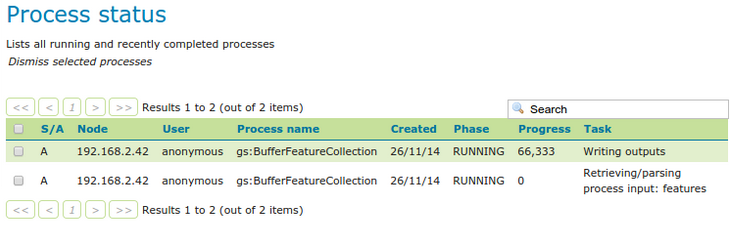
\includegraphics[width=\textwidth]{img/geoserver_status.png}
\caption{Process status page, source \cite{GS_docs}}
\label{fig:geoserver_status}
\end{figure}

\subsection{ZOO-Project}
\textit{ZOO-Project} is a WPS implementation writen in C, Python and Javascript. It is an open-source project released under MIT licence.
The platform is composed of several components:

\begin{itemize}
\item WPS Server - ZOO-kernel is a server-side implementation written in C.
\item WPS Services - ZOO-services is a set of ready-to-use web services based on libraries such as \textit{GDAL}, \textit{GRASS GIS}
or \textit{CGAL}.
\item WPS API - ZOO-API is a server-side Javascript API for creating and chaining WPS web services.
\item WPS Client - ZOO-client is a client-side Javascript library for interacting with WPS Services.
\end{itemize}

ZOO-Project is the first and in this time probably only one full implementation of the WPS 2.0.0 standard. Apart from \textit{GetCapabilities},
\textit{DescribeProcess} and \textit{Execute} operations from WPS 1.0.0 standard it also implements \textit{GetStatus}, \textit{GetResult}
and \textit{Dismiss} operations from WPS 2.0.0.

To comply WPS 2.0.0 ZOO-Project must support synchronous/asynchronous
%% ML: To store ... - ta veta zni divne
%% AL: Prepsano.
invocation with both HTTP-GET and HTTP-POST request. There is optional 
MapServer support so an output can be stored in MapServer catalog. It is convenient to publish
results directly as WMS, WFS or WCS resources.

\subsection{ArcGIS Server}
\textit{ArcGIS Server} is server-side GIS software developed by
\textit{Esri}. It is capable of creating and managing GIS Web
%% ML: exposing ?
%% AL: opraveno
services, applications and data. It allows exposing the analytic
capability of ArcGIS to web as a \textit{Geoprocessing service}. A
%%% ML: moc mi ta veta nedava smysl
%% AL: zkusil jsem to rozdelit, je to lepsi?
geoprocessing service consists of one or more geoprocessing tasks. 
A geoprocessing task can be any ArcGIS tool. It is possible to
publish Geoprocessing service with the WPS capabilities enabled,
however only WPS 1.0.0 standard is supported.

\begin{figure}[h!]
\centering

\includegraphics[width=0.3\textwidth]{img/Intro_esri.png}
\caption{Esri logo}
\label{fig:geoserver_status}
\end{figure}

All published services have specified the minimum and maximum number of available instances. These instances run on the container machines within processes. The isolation level determines whether these instances run in separate processes or shared processes. 
\begin{itemize}
\item \textit{High isolation}- Fig. \ref{fig:arcgis_isolation_low} - each instance runs in its own process. If something causes the process to fail, it will only affect the single instance running in it.
\item \textit{Low isolation} - Fig. \ref{fig:arcgis_isolation_high} allows multiple instances of a service configuration to share a single process, thus allowing one process to handle multiple concurrent, independent requests. This is often referred to as multithreading.
\end{itemize} 

\begin{figure}[h!]
\centering
\begin{floatrow}
\ffigbox{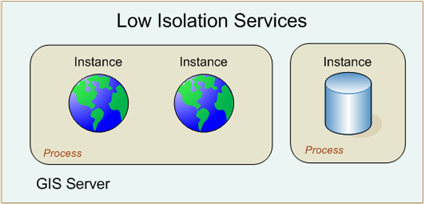
\includegraphics[width=0.5\textwidth]{img/arcgis_isolation_low.png}}{\caption{Low isolation, source \cite{AG_docs}}}{\label{fig:arcgis_isolation_low}}
\ffigbox{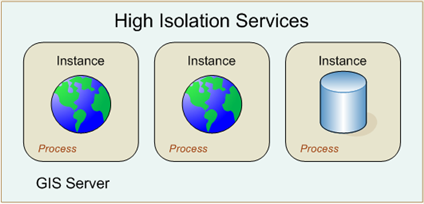
\includegraphics[width=0.5\textwidth]{img/arcgis_isolation_high.png}}{\caption{High isolation, source \cite{AG_docs}}}{\label{fig:arcgis_isolation_high}}
\end{floatrow}
\end{figure}

The advantage of low isolation is that it increases the number of concurrent instances supported by a single process. Using low isolation can use slightly less memory on your server. However, this improvement comes with some risk. If a process experiences a shutdown or crash, all instances sharing the process are destroyed. It is strongly recommended that you use high isolation.\cite{AG_docs}

\subsection{PyWPS}
PyWPS is a server-side implementation of the WPS standard written in Python. This project will be described in depth in the Sec. \ref{sec:PyWPS}.


\newpage
\part{PyWPS}

\newpage
\section{PyWPS}
\label{sec:PyWPS}
\subsection{History}
The origin of PyWPS started in 2006 as a student project. The first presentation was held at the FOSS4G 2006 conference in Lausanne titled 
‘GRASS goes to web: PyWPS’. During November 2006 the version 1.0.0 was released together with WUIW and Embrio projects that brought the
funcionality of GRASS GIS and general web interface able to handle any WPS server.\cite{PyWPS_presentation}\cite{PyWPS_web}

In 2007 PyWPS 2.0.0 was released supporting WPS standard 0.4.0. New
%% ML: a -> and?
%% AL: and
version improved stability and approached on the standard
implementation. It came with new WPS client and WPS plugin for
OpenLayers \footnote{\url{http://openlayers.org/}}.

Next year in 2008 PyWPS 3.0.0 was released with support for WPS 1.0.0. It was possible to run multiple WPS instances
with one PyWPS installation. This version had simple code structure and contained examples of processes. 

The newest version is PyWPS 4.0.0 from 2016 when PyWPS-4 branch was merged to official PyWPS repository as its master branch.
 New version is described in following Sec. \ref{sec:PyWPS4}.

\begin{figure}[h!]
\centering

\includegraphics[width=0.4\textwidth]{img/pywps_logo.png}
\caption{PyWPS project logo}
\label{fig:pywps_logo}
\end{figure}

\subsection{PyWPS 4.0}
\label{sec:PyWPS4}
%% ML: this -> these
%% AL: these
PyWPS-4 is the most current version of PyWPS. Rewriting from scratch involved these major changes:
\begin{itemize}
\item It is written in \textit{Python 3} with backward support for Python 2.7.
\item It utilizes native Python bindings to existing projects (GRASS GIS).
\item New popular formats like \textit{GeoJSON}, \textit{KML} or \textit{TopoJSON} are reflected and their support is provided.
\item PyWPS project has changed the license from \textit{GNU/GPL} to \textit{MIT}.
\item PyWPS 4.0 is implemented using the \textit{Flask} framework.
\item A C-based XML parser \textit{Lxml} is used to handle XML files.
\item \textit{OWSLib} structures are used for some data types.
\end{itemize}

\subsection{PyWPS-demo}
\label{sub:demo}
PyWPS-demo is a small side project distributed with PyWPS. It is a simple demo instance of PyWPS server running on 
\textit{Flask}\footnote{\url{http://flask.pocoo.org/}}. Flask is a microframework for web applications in Python. 
Flask provides built-in development server and debugger and RESTful request dispatching. Starting PyWPS-demo server with Flask
is very simple and can be done with command in Lst. \ref{lst:demo_start}. After starting the PyWPS-demo server the PyWPS homepage can be 
visited at: \url{http://localhost:5000}.

\bigskip
\begin{lstlisting}[basicstyle=\small,caption={Starting PyWPS-demo server},label={lst:demo_start}]
python3 demo.py
\end{lstlisting}

PyWPS-demo comes with several demo processes:
\begin{itemize}
\item \textit{area.py} - Process calculates area of given polygon.
\item \textit{bboxinout.py} - Process transforms bounding box to another EPSG.
\item \textit{buffer.py} - Process returns buffers around the input features, using the GDAL library.
\item \textit{centroids.py} - Process returns a GeoJSON with centroids of features from an uploaded GML.
\item \textit{feature\_count.py} - Process counts the number of features in an uploaded GML.
\item \textit{grassbuffer.py} - Process uses the  GRASS GIS \textit{v.buffer} module to generate buffers around inputs.
\item \textit{sayhello.py} - Process returns a literal string output with Hello plus the inputed name.
\item \textit{sleep.py} - Process will sleep for a given delay or 10 seconds if not a valid value.
\item \textit{ultimate\_question.py} - The process gives the answer to the ultimate question of "What is the meaning of life?"
\end{itemize}

Except these example processes the demo offers also example configuration file. Configuration file contains several parameters in
these four sections:
\begin{itemize}
\item \textit{metadata} - parameters containing information for metadata creation.
\item \textit{server} - definition of path to workdir and output directories, maximum number of parallel running or stored processes. 
\item \textit{logging} - logging level setting, path to log file and log database.
\item \textit{grass} - GRASS settings.
\end{itemize}



\newpage
\section{Process isolation in PyWPS}
\subsection{Asynchonous requests}
Right now in PyWPS 4.0 version a PyWPS server instance is able to run
multiple concurrent processes in parallel. The server is configured
%% ML: maximal amount(s) se opakuje dvakrat po sobe
%% AL: pouzito maximum, je to lepsi?
for maximal amounts of concurrently running processes at the same time
and for maximum of waiting processes in a queue, to later
start their execution once new slots are available. If the new Execute
request is received and the maximal amount is exceeded, the request is
rejected and user is informed in response (see
Lst. \ref{lst:Isolation_rejected}).

\begin{lstlisting}[basicstyle=\small,caption={Resource exceeded exception},label={lst:Isolation_rejected}]
<?xml version="1.0" encoding="UTF-8"?>
<ows:ExceptionReport xmlns:ows="http://www.opengis.net/ows/1.1" version="1.0.0">
    <ows:Exception exceptionCode="ServerBusy">
        <ows:ExceptionText>
            Maximum number of parallel running processes reached. Please try later.
        </ows:ExceptionText>
    </ows:Exception>
</ows:ExceptionReport>
\end{lstlisting}

To facilitate the management of concurrent processes, process metadata
%% ML: dve vety za sebou zacinaji stejne: This database...
%% AL: opraveno
are stored into a local database. This database is used for logging
and saving waiting Execute requests in the queue and invoking them
later on. The database will also enable the implementation of
pausing, releasing and deleting running process. These features will
allow PyWPS to comply with WPS version 2.0.0.

\subsection{Current state}
\label{subsec:current_state}
At the beginning of every process execution its own temporary directory \textit{workdir} is created. During the execution
temporary files and continuous outputs are stored in this directory. After successful execution final outputs are
moved to \textit{outputs} directory. Both directories \textit{outputs} and \textit{workdir} are configurable and user can
change path to them.

\bigskip
\begin{lstlisting}[basicstyle=\small,caption={pywps.cfg - mode parameter}]
[processing]
mode=multiprocessing
\end{lstlisting}

Current version of PyWPS offers two solutions for running parallel processes:
\begin{itemize}
\item Multiprocessing
\item Job Scheduler Extension\footnote{Job Scheduler Extension is currently only in \textit{develop} branch of PyWPS.}
\end{itemize}

If the execute request is sent asynchronously the type of process constructor is chosen depending on configuration
parameter \textit{mode} in section \textit{processing} which is by default \textit{multiprocessing} or can be changed 
to \textit{scheduler}.

%% ML: je tato ukazka kodu opravdu nutna?
%% AL: smazano

\paragraph{Multiprocessing}
By default for  processes running in the background, the Python \textit{multiprocessing} module is used – 
this makes it possible to use PyWPS on the Windows operating system too.

\begin{figure}[h!]
\centering
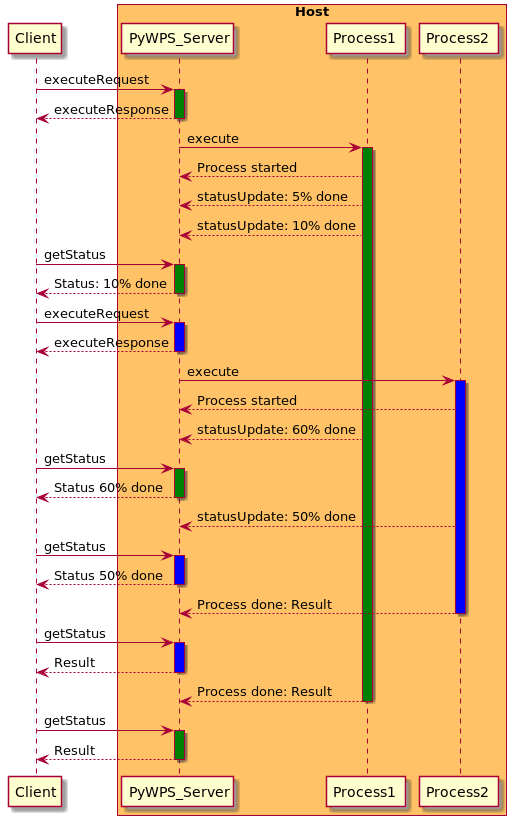
\includegraphics[width=0.7\textwidth]{img/Diag_multiprocessing.png}
\caption{Sequence diagram: Multiprocessing}
\label{fig:Diag_multiprocessing}
\end{figure}

The number of processes running in parallel is configirable by parameter \textit{parallelprocesses} of section \textit{server} in 
configuration file. In the Fig. \ref{fig:Diag_multiprocessing} two running processes are shown. A client sends an Execute request to
a server. Server sends back to the client an ExecuteResponse that \textit{Process1} (green in the figure) was accepted and starts its 
execution. During the execution the process updates its status. The interval of status updates depends on the code of the Process1.
Process1 must support status update otherwise it cannot be run in asynchronous mode.

During the execution of Process1 server receives another Execution request. It sends back the Execution response and starts the execution
of \textit{Process2} (blue in the figure). Separated Python \textit{Process}\footnote{Explanation of term Python \textit{Process} and its
differences to \textit{Thread} is in next paragraph.} is created. Both of the processes run on the host machine, however both have own memory
space. Their executions run concurently and client can request their status. In the figure, the Process2 ended first and client can retrieve
the result from the server. Once the Process1 ends, the client can retrieve its result from the server as well.

It is important to say that in case of multiprocessing, processes run concurently with its own memory space, nevertheless they are not isolated.
They run on the same host machine and share the resources. There are even methods like \textit{Pipe()} that enable communication between 
processes.

\paragraph{Process vs Thread} In Python there are two ways to achieve \textit{pararellism}. It is \textit{multiprocessing}
\footnote{\url{https://docs.python.org/3/library/multiprocessing.html}} with using processes and \textit{threading}\footnote{\url{https://docs.python.org/3/library/threading.html}} with threads. The main difference is that threads run in the same memory space, while processes
have separate memory. Multiprocessing takes advantages of multiple CPUs and cores while threads are more lightweighted and have low memory
footprint. In case of PyWPS asynchronous requests, for every execution its own process with its own memory space is created.

\paragraph{Job Scheduler Extension}
PyWPS scheduler extension offers possibilities to execute asynchronous processes out of the WPS server machine.
This extension enables to delegate execution of processes to a scheduler system like \textit{Slurm}, \textit{Grid Engine} 
and \textit{TORQUE} from Adaptive Computing. These schedular systems are usually located at \textit{High Performance Compute (HPC)}
centers.

\begin{figure}[h!]
\centering
\begin{floatrow}
\ffigbox{
\includegraphics[width=0.33\textwidth]{img/Isolation_grid.jpg}}{\caption{Grid Engine}}{\label{fig:Isolation_grid}}
\ffigbox{
\includegraphics[width=0.25\textwidth]{img/Isolation_slurm.png}}{\caption{Slurm}}{\label{fig:Isolation_slurm}}
\end{floatrow}
\end{figure}

\begin{figure}[h!]
\centering

\includegraphics[width=0.33\textwidth]{img/Isolation_torque.png}
\caption{TORQUE}
\label{fig:Isolation_torque}
\end{figure}
\bigskip

The PyWPS scheduler extension uses the Python \textit{dill} library to dump and load the processing job to/from filesystem. The batch script executed on the scheduler system calls the PyWPS \textit{joblauncher} script with the dumped job status and executes the job (no WPS service running on scheduler). The job status is updated on the filesystem. Both the PyWPS service and the joblauncher script use the same PyWPS configuration. The scheduler assumes that the PyWPS server has a shared filesystem with the scheduler system so that XML status documents and WPS outputs can be found at the same file location. The interaction diagram how the communication between PyWPS and the scheduler works is displayed in Fig. \ref{fig:Isolation_interaction}.

\bigskip
\begin{figure}[h!]
\centering
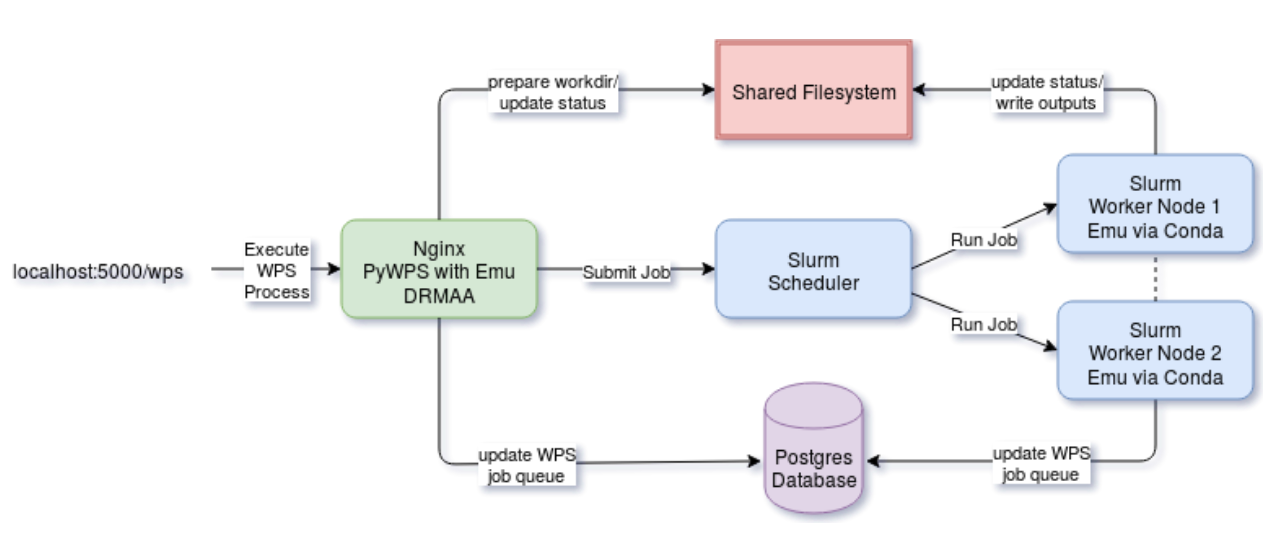
\includegraphics[width=\textwidth]{img/Isolation_slurm_usage.png}
\caption{Example of PyWPS scheduler extension usage with Slurm, source: \cite{PyWPS_docs}}
\label{fig:Isolation_slurm_usage}
\end{figure}

\begin{figure}[h!]
\centering
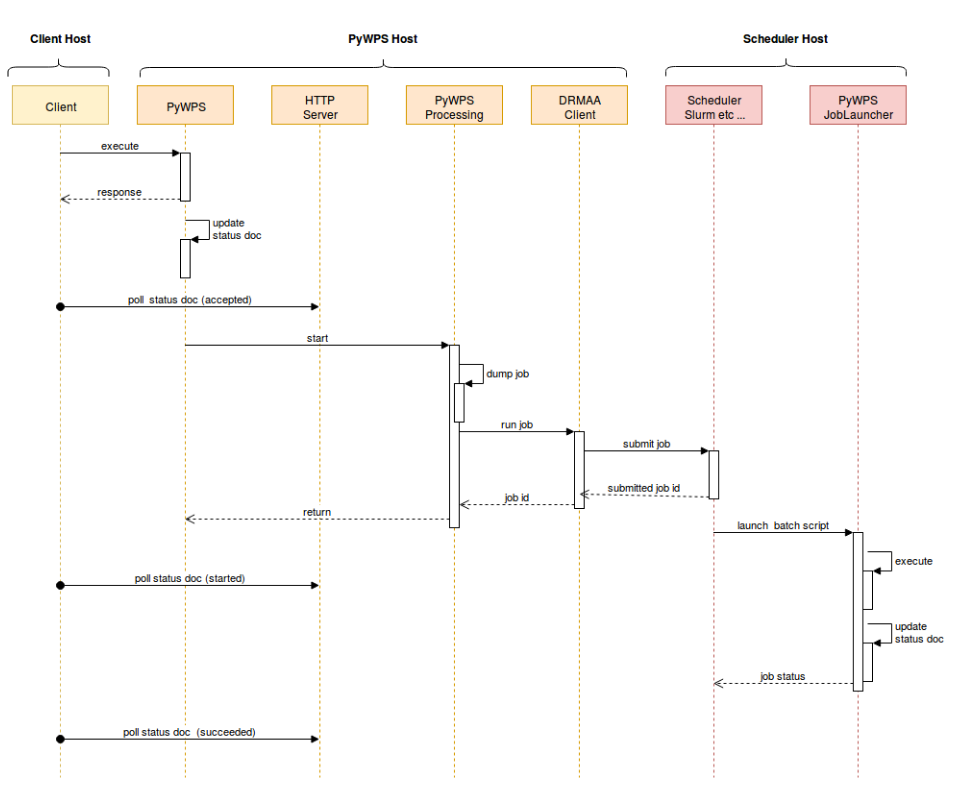
\includegraphics[width=\textwidth]{img/Isolation_interaction.png}
\caption{Communication between PyWPS and scheduler, source: \cite{PyWPS_docs}}
\label{fig:Isolation_interaction}
\end{figure}

%% ML: upresnit nadpis
%% AL: upresneno
\subsection{Possible solutions for process isolation}
In previous section there were described two mechanisms for running parallel processes. Nevertheless in case of Python module
\textit{Multiprocessing} the processes are not really isolated. They run concurrently but they can share resources and there are 
even methods like \textit{Pipe()} that enables communication between processes.

%% ML: depends?
%% AL: depends
On the other hand \textit{Job Scheduler Extension} depends on
\textit{dill} library as well as on some external scheduler systems
like \textit{Slurm}, \textit{Grid Engine} or \textit{TORQUE}.

%% MK: v tomto odstavce se to hemzi "some of them"
%% AL: prepsano
\bigskip In this section there are described some other
solutions. Some were suggested by PyPWS developers with
encouragement to make a feasible study. Others were discovered
during research on the internet forums like StackOverflow and few of
them were referenced in the documentation of other projects. During
the research two requirements were considered.

\begin{itemize}
\item The solution provides a mechanism for full isolation. This is a must-have requirement.
\item The solution provides a mechanism for start/pause/stop process execution. This is a nice-to-have requirement as this functionality
will be required to comply WPS 2.0.0 standard.
\end{itemize}

\noindent
Finnaly these solutions were considered:
\begin{itemize}
\item Celery
\item Docker
\item psutil
\item SandboxedPython
\item VM
\end{itemize}

\subsubsection{Celery}
\textit{Celery} is a task queue system written in Python. It helps to distribute work across threads and even machines. Basic term is
a \textit{task}. A task is a unit of work and it is an input into the task queue. The task queue is constantly monitored for new 
work to perform.

To communicate between client and workers Celery uses a \textit{broker}. The communication is via messages. To initiate a task the
client adds a message to the queue and the broker then delivers the message to a worker. Multiple workers and brokers can be added
so there is assured high availability and horizontal scaling.

Celery provides worker remote control client in class
\textit{celery.app.control.Control}. The class offers following functions:
\begin{itemize}
\item\textbf{revoke} - Tell all (or specific) workers to revoke a task by id. If a task is revoked, the workers will ignore the task and not execute it after all.
\item\textbf{shutdown} - Shutdown worker(s).
\item\textbf{terminate} - Tell all (or specific) workers to terminate a task by id.
\end{itemize}

\subsubsection{Docker}
\textit{Docker} is one of the most used technology regarding containerization. This technology is described in depth in Sec. \ref{sec:Docker}

\subsubsection{psutil}
\textit{psutil} is Python library for process and system management. It handles system monitoring, limiting process resources
and the management of running processes. Its implementation is based on UNIX command line tools. psutil offers functions applied
to these sections:
\begin{itemize}
\item CPU - functions for CPU statistics such as CPU utilization percentage, frequency and others. 
\item Memory - functions for system memory usage and swap memory statistics.
\item Disks - functions for disk statistics such as disk usage or disk IO operations counter.
\item Network - functions for network IO operations or network connection statistics.
\item Sensors - functions for statistics about fans, battery or hardware temperature.
\item Others - functions for boot time and users statistics.
\item Processes - functions will be described in detail later.
\end{itemize}

\paragraph{Processes} - Class \textit{psutil.Process} represents an OS
%% ML: vysvetlit pid (poznamka pod carou, ci jinak)
%% AL: mam to ve zkratkach, ale pridal jsem i poznamku
process with given pid. The class is bound with a process via its
PID\footnote{\textit{PID} is a process identifier. It is a number used by operating system to uniquely identify an active process.}. The \textit{Process} class offers these methods for
starting/pausing:
\begin{itemize}
\item suspend() - The method suspends a process using \textit{SIGSTOP} signal.
\item resume() - The method resumes a process using \textit{SIGCONT} signal.
\item terminate() - The method terminates a process using \textit{SIGTERM} signal.
\item kill() - The method kills a process using \textit{SIGKILL} signal.
\end{itemize}

\subsubsection{Sandboxed Python}
The general goal of a sandbox is to run applications securely inside isolated environment they cannot escape from and
affect other parts of the system. Developers use them to run untrusted code inside. It is quite difficult to develop
fully sandboxed solution due to Python complexity. The basic problem is that Python introspection allows several ways
to escape out of the sandbox. True security requires an overall design with many security considerations included. Some
of the projects that can run Python code in a sandbox are:
\begin{itemize}
\item PyPy
\item Jython
\end{itemize}

\paragraph{PyPy} PyPy is Python interpreter written in RPython that implements full Python language and very closely 
emulates the behavior of CPython. PyPy offers fully portable sandboxing feature similar to OS-level sandboxing (e.g. SECCOMP).
It is not sandboxing at the Python language level so it does not put any restriction on any Python functionality.

Untrusted Python code that is intended to be sandboxed is launched in a subprocess, that is a special sandboxed version of PyPy.
All its inputs/outputs are not directly performed but are serialized to a stdin/stdout pipe. The outer process reads the pipe 
and afterward decides which commands are allowed.

\paragraph{Jython} Jython is Python language interpreter for Java. Java offers strong sandboxing mechanisms. The security 
facility in Java that supports sandboxing is the \textit{java.lang.SecurityManager}. By default, Java runs without a 
SecurityManager.

\paragraph{pysandbox} A prove, that it is very difficult to develop some kind of sandbox with all security holes 
considered, could be a project  \textit{pysandbox}\footnote{\url{https://github.com/vstinner/pysandbox}}. After working 
on it for 3 years, during which the project was used on various production servers by other developers, its author 
declared that the project is broken by
design. In his post to the python-dev mailing list \cite{PyDev_ML} the author explained that with every vulnerability 
founded it became more difficult to actually write a real code:

\textit{
"To protect the untrusted namespace, pysandbox installs a lot of
different protections. Because of all these protections, it becomes
hard to write Python code. Basic features like "del dict[key]" are
denied. Passing an object to a sandbox is not possible to sandbox,
pysandbox is unable to proxify arbitary objects.}

\textit{
For something more complex than evaluating "1+(2*3)", pysandbox cannot
be used in practice, because of all these protections. Individual
protections cannot be disabled, all protections are required to get a
secure sandbox."}

\subsubsection{Virtual Machine/Vagrant}
Using full virtualization for process isolation is mentioned here but in fact it is hard to imagine this solution could work
in practice. \textit{Vagrant} is a tool for managing and building virtual machines. It provides a way how to manage various virtual 
machines in an automatized way e.g. using scripts. There also exists a Python package \textit{python-vagrant} that offers 
Python bindings for interacting with Vagrant.

However in our use-case using Vagrant would mean that for every process execution a separate virtual machine would
be created. Depending
on the process algorithm complexity the process execution can last from milliseconds to hours or days. On the other hand building 
a virtual machine and booting into it last at least few seconds. That is why it is hard to imagine using virtual machine, which takes
few seconds to boot up, to isolate process, which execution lasts less than a second.

\newpage
\section{Docker}
{sec:Docker}
\textbf{Containerization} is a lightweight alternative to full machine virtualization. It involves encapsulating an application 
into a container with its own operating environment. It helps to run a containerized application on any physical machine without any
worries about dependencies. The origin of containerization lies in the \textit{LinuX Containers {LXC}} format. Containerization
works only in Linux environments and can run only Linux applications.

\begin{figure}[h!]
\centering

\includegraphics[width=0.33\textwidth]{img/Docker_logo}
\caption{Docker logo}
\label{fig:Docker_logo}
\end{figure}

Docker is not the only technology for containerization. Other alternatives exist, it is \textit{Kubernets}, \textit{CoreOS rkt}, 
\textit{Open Container Initiative (OCI)}, \textit{Canonical's LXD}, \textit{Apache Mesos and Mesosphere} and many others. 
However Docker is a leader on the field of containerization and with most public traction is de facto considered as a~container standard.
That's why the Docker was chosen for this thesis as a~container technology. So from this point on any term \textit{container} refers to
Docker container.

\begin{figure}[h!]
\centering
\begin{floatrow}
\ffigbox{
\includegraphics[width=0.2\textwidth]{img/Docker_kubernetes.png}}{\caption{Kubernetes}\label{fig:Docker_kubernetes}}
\ffigbox{
\includegraphics[width=0.2\textwidth]{img/Docker_rkt.png}}{\caption{CoreOS rkt}\label{fig:Docker_rkt}}
\end{floatrow}
\end{figure}

\begin{figure}[h!]
\centering
\begin{floatrow}
\ffigbox{
\includegraphics[width=0.13\textwidth]{img/Docker_lxd.png}}{\caption{Canonical's LXD}\label{fig:Docker_lxd}}
\ffigbox{
\includegraphics[width=0.25\textwidth]{img/Docker_mesos.jpg}}{\caption{Apache mesos}\label{fig:Docker_mesos}}
\end{floatrow}
\end{figure}

\paragraph{Docker} is a Linux container technology that allows package and ship applications and everything it needs to execute into a standard
format, and run them on any infrastructure.

\subsection{Virtual machine vs. Docker container}
Both virtual machines and Docker containers are two ways how to deploy multiple, isolated applications on a single platform. They
both offer a way to isolate an application and its dependencies into a self-contained unit that can run anywhere. They both offer
some kind of virtualization. They differ in architecture, see Fig. \ref{fig:Docker_VM}, \ref{fig:Docker_container}.

\begin{figure}[h!]
\centering
\begin{floatrow}
\ffigbox{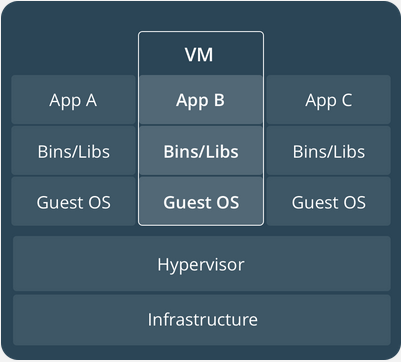
\includegraphics[width=0.495\textwidth]{img/Docker_VM.png}}{\caption{Virtual machine architecture, source \cite{Docker_docs}}\label{fig:Docker_VM}}
\ffigbox{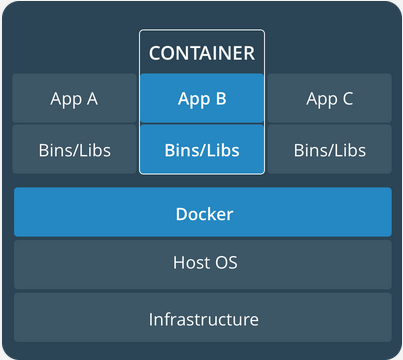
\includegraphics[width=0.5\textwidth]{img/Docker_container.png}}{\caption{Containers architecture, source \cite{Docker_docs}}\label{fig:Docker_container}}
\end{floatrow}
\end{figure}

\subsubsection{Virtual machine}
Let's start with a virtual machine (Fig. \ref{fig:Docker_VM}) and its layers description from the bottom up:
\begin{itemize}
\item \textit{Infrastructure} - It can be a PC, developer's laptop, a
  physical server in datacenter but as well a virtual private server
  %% ML: nemelo by tady byt misto EC2 -> AWS (jako zastresujici zalezitost)?
  %% AL: opraveno
  in the cloud as Microsoft Azure or Amazon Web Services.
\item \textit{Host OS} - Host operating system. In case of native
  hypervisor this layer is missing. In case of hosted hypervisor it is
  probably some distribution of Linux, Windows or MacOS.
\item \textit{Hypervisor} - Also called virtual machine monitor (VMM). It allows hosting several different virtual machines
on a single hardware. There are two types of hypervisors:
\begin{itemize}
\item Type 1 -  Also called \textit{bare metal} or \textit{native}. This type is run on the host's hardware to control it as well as manage 
the virtual machines on it. It is much faster and more efficient. This type hypervisors are KVM, Hyper-V or HyperKit.
\item Type 2 - So called \textit{embedded} or \textit{hosted} hypervisors. These hypervisors are run on a host OS as a software. They are slower
and less efficient on the other hand they are much easier to set up. It includes VirtualBox or VMWare Workstation.
\end{itemize}
\item \textit{Guest OS} - Guest operating system. Each VM requires own guest operating system which is controlled by the hypervisor. Each 
guest OS needs its own CPU and memory resources and starts on hundreds of megabytes in size.
\item \textit{Bins/Libs} - Each guest OS needs various binaries and libraries for running the application. It can be \textit{python-dev} or \textit{default-jdk} packages as well as personal packages to run the application.
\item \textit{Application} - The application source code that is desired to be run isolated. Therefore each application or each version of the application has to be run inside of its own guest OS with own copy of bins and libs. 
\end{itemize}

\subsubsection{Docker container}
\noindent
Now, what is different regarding containers (Fig. \ref{fig:Docker_container}):
\begin{itemize}
\item \textit{Infrastructure} - PC, laptop, physical or virtual server.
\item \textit{Host OS with container support} - Any OS capable of run Docker. All major distributions of Linux are supported and there are ways
to run Docker even on MacOs and Windows too.
\item \textit{Docker engine} - Also called Docker daemon. It is a service that runs in the background on host operating system. It manages all interaction with containers.
\item \textit{Bins/Libs} - Binaries and libraries required by the application. They get built into special packages called \textit{Docker images}.
The Docker daemon runs those images.
\item \textit{Application} - Each application and its library dependencies get packed into the same Docker image. It is managed independently by the Docker daemon. 
\end{itemize}

\noindent
But the architecture is not the only one difference:
\begin{itemize}
\item Docker uses Docker daemon to manage containers, hypervisor manages virtual machines.
\item The Docker daemon communicates directly with host OS and manage resources for each container.
\item VMs usually boot up in a minute and more, containers start in seconds.
\item Docker virtualizes operating systems, using VMs is hardware virtualization.
\item VM and container vary in size. VMs start at hundreds of megabytes. A container can be smaller than one megabyte.
\item Containers share the kernel although they are isolated. VMs are monolithic and stand-alone.
\end{itemize}

\subsection{Dockerfile}
Dockerfile is a core file that contains the instruction to be performed when an image is built. It usually consists of commands to install packages, calls to other scripts, setting environmental variables, adding files or setting permissions. In Dockerfile there is also defined what image is to be used as a base image for the build.

\paragraph{Dockerfile instructions}
\begin{itemize}
\item \textit{FROM} - The FROM instruction defines the base image for next instructions and initializes a new build stage. Every Dockerfile
has to start with FROM command. The only exception is ARG command which can be before FROM command.
\item \textit{ARG} - The ARG instruction defines a variable that users can pass at build-time to the builder.
\item \textit{ENV <key>=<value>} - The ENV instruction sets the environment variables. It is key-pair value. 
\item \textit{LABEL} - The LABEL instruction adds metadata to an image. A LABEL is a key-value pair. It can be anything from version number to a description.
\item \textit{ADD <src> <dest>} - The ADD instruction copies files or directories from source and adds them at the destination path. It also unzips or untars files when added.
\item \textit{COPY <src> <dest>} - Similar to the ADD instruction it copies files or directories from source and adds them to the destination path. This command doesn't provide any kind of decompression.
\item \textit{RUN <command>} - The RUN instruction will execute any defined command and commit the results.
\item \textit{CMD ["executable","param1","param2"]} - The CMD instruction provides defaults for an executing container. It can include an
executable. In case the executable is omitted the CMD instruction must be used together with the ENTRYPOINT instruction. There can be only
one CMD instruction in Dockerfile. In case there is more CMD the last one will be used.
\item \textit{ENTRYPOINT} - The ENTRYPOINT defines a container configuration that will run as executable.
\item \textit{WORKDIR /path/to/dir} - The WORKDIR instruction sets the working directory for any RUN, CMD, COPY and ADD instruction that follows in Dockerfile.
\item \textit{EXPOSE} - The EXPOSE instruction informs Docker that the container listens on the specified network ports at runtime.
\item \textit{VOLUME} - The VOLUME instruction creates a mount point with the specified name and marks it as holding externally mounted volumes from the native host or other containers.
\end{itemize}

Except for the FROM instruction, all the instructions can be defined from the command line when starting docker container. There are more Dockerfile instructions however they are not relevant to this thesis as there are never used in practical part. A Dockerfile, which was created during the work on the thesis, is available at App. \ref{app:dockerfile}.

%% ML: chybi tu odkaz na appendix
%% AL: odkaz pridan

\newpage
\part{Implementation}

\newpage
\section{Implementation introduction}

% ML: ta kapitola je spis shrnuti zmen nez uvod :-) Ale uz to nech, tak jak to je
\subsection{pywps-demo}
During the implementation the \textit{pywps-demo}
(Sec. \ref{sub:demo}) running on \textit{Flask} framework was
used. This demo server instance runs on host machine server at port
5000 as well as the image built from its Dockerfile is used for every
container creation. For developing purpose some sections were added to
configuration file as well some minor changes for instance in server
routing were made. The diff file to pywps-demo is in
App. \ref{app:pywps-demo}.

\subsubsection{pywps-demo Dockerfile}
\textit{pywps-demo} is also available as a Dockerfile and as mentioned
the image built from this Dockerfile is used for container creation.
Before the work on this thesis started, the pywps-demo project had
offered two dockerfiles, both based on \textit{alpine Linux}
distribution. The first one \textit{pywps-flask} was the default
implementation using only Flask while the second one \textit{nginx}
implements pywps using Nginx and Green unicorn as WSGI server. During
the implementation only the \textit{pywps-flask} Dockerfile was
used. However it was necessary to modify the Dockerfile because it did
%% ML: je nekde vysvetleno, proc je potreba GDAL, pokud ano, tak zde chybi reference
%% AL: pridano vysvetleni
not contain \textit{GDAL} library which is required for most of the
demo processes that \textit{pywps-demo} offers.

During implementaion a new version of Dockerfile with
support of GDAL was created in collaboration with PyWPS
developers. There were some issues with \textit{Xerces} libraries
whose packages are not available for alpine distribution and its
manual instalation was necessary. The newly-created Dockerfile is
%% ML: ta posledni veta zni divne, v odstavci se opakuje casteji "work
%% on this thesis"
%% AL: prepsano
available in App. \ref{app:dockerfile}. At the time of finishing this
thesis pywps-demo offers dockerfiles based on \textit{alpine} and
\textit{ubuntu} Linux distribution.

\subsection{OWSLib}
\label{sub:owslib}
A Python package \textit{OWSLib} was used for forwarding requests from
PyWPS server instance running on host machine to PyWPS server instance
%% ML: detailly?
%% AL: 
running inside a Docker container. Some bug fixing which is
mentioned in Sec.\ref{sub:Container_execute} was necessary. Complete
%% ML: Byly ty upravy zacleneny do OWSlib, pokud ano, tak to zmin
%% AL: Pull request jsem zatim neresil.
%% ML: v zaveru ale o pull requestu mluvis
diff is available in App. \ref{app:owslib}.

\subsection{PyWPS}
Most changes have been done in core PyWPS project. Almost all changes were made in \textit{processing} module. To this module new file
\textit{container.py} containing the \textit{Container} class was added. Complete diff is available at App. \ref{app:pywps}.

\newpage
\section{Operations overview}
\label{sec:operations_ov}
PyWPS in current version 4.0.0 implements all mandatory operations: \textit{Execute}, \textit{GetCapabilities}, \textit{DescribeProcess}.
Operations are handled by corresponding methods \textit{execute()}, \textit{get\_capabilities()} and \textit{describe()} in \textit{Service} class. 

However both \textit{GetCapabilities} and \textit{DescribeProcess}
operations run in synchronous mode only. After sending a request, a
client receives back GetCapabilities or DescribeProcess response (both
detaily described in \ref{para:GetCapa_response} and
\ref{para:DesribeProc_response}). Both operations return only
information or description about process but do not trigger the
execution of the process. It is supposed the response to
GetCapabilities and DescribeProcess is returned almost immediately.
During the GetCapabilities and the DescribeProcess operations a
process execution is not started and therefore there is no starting
%% ML: ta posledni veta zni divne
%% AL: opraveno
process to be isolated. That is why whole contribution of this thesis
only applies to \textit{Execute} operation.

%% ML: chybi zdroj, pokud je to Tvuj diagram, tak to uved (napr. (source: author))
%% AL: ok
\begin{figure}[h!]
\centering
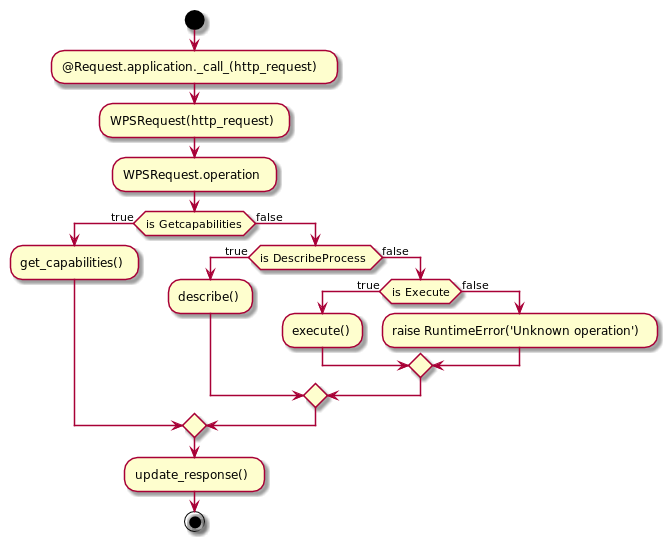
\includegraphics[width=0.9\textwidth]{img/Diag_operations.png}
\caption{PyWPS operations activity diagram, source: author}
\label{fig:Diag_operations}
\end{figure}

\section{Execute operation}
\subsection{Service.execute()}
As mentioned in previous section Sect. \ref{sec:operations_ov}, \textit{Execute} operation is handled by \textit{execute()} method.
Inputs for the method are:
\begin{itemize}
\item \textit{identifier} (string) - a name of the process which execution is requested and which is supported by WPS server.
\item \textit{wps\_request} (WPSRequest object) - an object containing original HTTP request.
\item \textit{uuid} (integer) - unique identifier of process execution.
\end{itemize}

%% ML: opet: zdroj
%% AL: ok
\begin{figure}[h!]
\centering
\begin{floatrow}
\ffigbox{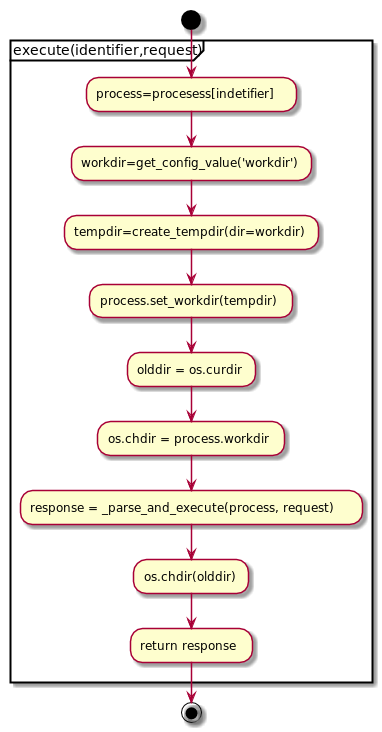
\includegraphics[width=0.4\textwidth]{img/Diag_service_execute.png}}{\caption{Activity diagram: method \textit{Service.execute()}, source: author}\label{fig:DiagServiceExecute}}
\ffigbox{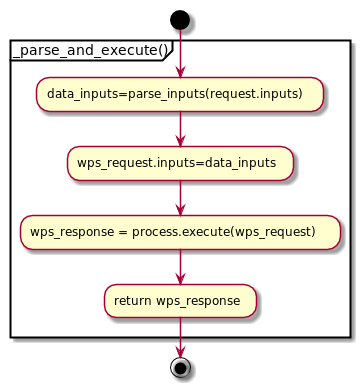
\includegraphics[width=0.4\textwidth]{img/Diag_service_parse_execute.png}}{\caption{Activity diagram: method \textit{Service.\_parse\_and\_execute()}, source: author}\label{fig:DiagServiceParseExecute}}
\end{floatrow}
\end{figure}

The flowchart of the process execution is displayed in Fig. \ref{fig:DiagServiceExecute}. 
At first a deepcopy of the process instance is created so that processes cannot override each other. Then a temporary working directory \textit{workdir} is created and set as a current workdir for the process execution. To the workdir all input files are
copied as well as all temporary files and outputs are stored here. Then the method \textit{\_parse\_and\_execute()} is called (see
Fig. \ref{fig:DiagServiceParseExecute}). Here the inputs are parsed, in case of a web-referenced input the data are downloaded to workdir, in case of data sent within a request the data are saved into a file in workdir. The process execution afterward runs in \textit{Process.execute()} method. This method returns a \textit{wps\_response} - an instance of \textit{WPSReponse} object.

\subsection{Process.execute()}
The method \textit{execute()} of class \textit{Process} contains crucial if-statement where is decided whether the process will be
run in asynchronous or synchronous mode. Running in asynchronous mode can be enforced by setting both attributes \textit{status} and \textit{storeExecuteResponse} of the \textit{ResponseDocument} element in the ExecuteRequest XML to True.

\newpage
\begin{lstlisting}[basicstyle=\small,caption={ReponseForm element of ExecuteRequest XML},language=XML,label={lst:Execute_ResponseForm}]
<wps:ResponseForm>
 <wps:ResponseDocument status="true" storeExecuteResponse="true">
  <wps:Output asReference="true">
   <ows:Identifier>buff_out</ows:Identifier>
  </wps:Output>
 </wps:ResponseDocument>
</wps:ResponseForm>
\end{lstlisting}
\bigskip 

No matter whether the process runs synchronously or asynchronously there is always a control how many parallel processes are currently
running. The number of the maximum of concurrently running processes can be configured. If the process is asynchronous and the number of currently running processes exceeds the maximal number, the process is stored and its execution is started lately. In case of the synchronous process the \textit{ServerBusy} exception is raised. If the number of processes is smaller than the maximal number of 
concurrent processes, the process can be executed. In synchronous mode the \textit{\_run\_process()} is called, in asynchronous mode the method \textit{\_run\_async()} is called. The activity diagram of the \textit{Process.execute()} is displayed in Fig.\ref{fig:Diag_process_execute}.

%% ML: zdroj?
%% AL: ok
\begin{figure}[h!]
\centering
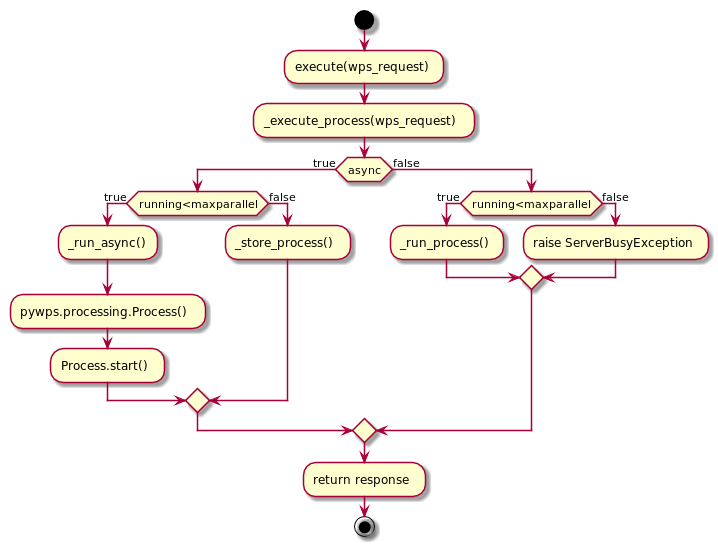
\includegraphics[width=0.9\textwidth]{img/Diag_process_execute.png}
\caption{\textit{Activity diagram: Process.execute()}, source: author}
\label{fig:Diag_process_execute}
\end{figure}

\subsection{Processing module}

%% ML: code -> operations ?
%% AL: asi lepsi operations
Until now the operations described in this thesis was not
modified. Requirements which have been considered during the
implementation of Docker technology were that the source code will
be modified slightly, the process isolation will be easily inserted and
the project structure will be kept the same. Keeping this in mind
changes in source code were made only in \textit{processing} module.

As mentioned in Sec. \ref{subsec:current_state}, PyWPS uses solely the Python package \textit{Multiprocessing} in production version.
In develop branch there is also \textit{Scheduler} extension as one of the option for multiprocessing. In this thesis another option 
\textit{Docker} for processing was added. The desired option for processing can be configured in configuration file via parameter \textit{mode} in section \textit{processing} (see Lst. \ref{lst:Mode_config}), possible values are:
\begin{itemize}
\item docker - new option
\item scheduler
\item multiprocessing - default option
\end{itemize}

\bigskip
\begin{lstlisting}[basicstyle=\small,caption={Processing mode configuration},language=XML,label={lst:Mode_config}]
[processing]
mode=docker/scheduler/multiprocessing
\end{lstlisting}

%% ML: zdroj
%% AL: ok
\begin{figure}[h!]
\centering
\begin{floatrow}
\ffigbox{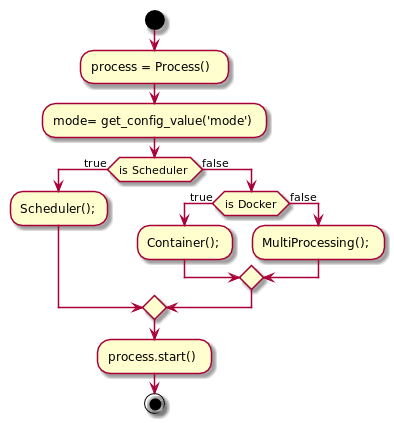
\includegraphics[width=0.48\textwidth]{img/Diag_run_async.png}}{\caption{Activity diagram: Method \textit{Process.\_run\_async()}, source: author}}{\label{fig:Diag_run_async}}
\ffigbox{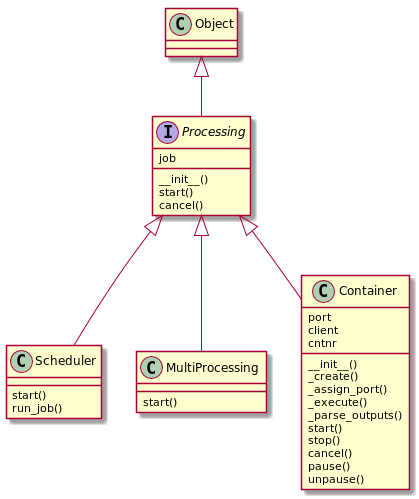
\includegraphics[width=0.48\textwidth]{img/Diag_class_processing.png}}{\caption{Class diagram: \textit{Processing} class, source: author}}{\label{fig:Diag_class_proc}}
\end{floatrow}
\end{figure}

\bigskip
The whole Docker implementation is in \textit{Container.py} module. The class \textit{Container} handles containers creation, interaction with
server, file-system mounting and all container management.

\newpage
\section{\textit{Container} class}
The main idea of process isolation using Docker is quite simple. For every process execution one separate Docker container is created.
Instead of starting process execution on the host PyWPS server after receiving ExecuteRequest from the client, the ExecuteRequest is
forwarded to PyWPS server running inside Docker container. The process execution runs inside the container. After successful process
execution the outputs are available at the host server. The host server and the container share the same process workdir at filesystem.

%% ML: zdroj
%% AL: ok
\bigskip
\begin{figure}[h!]
\centering
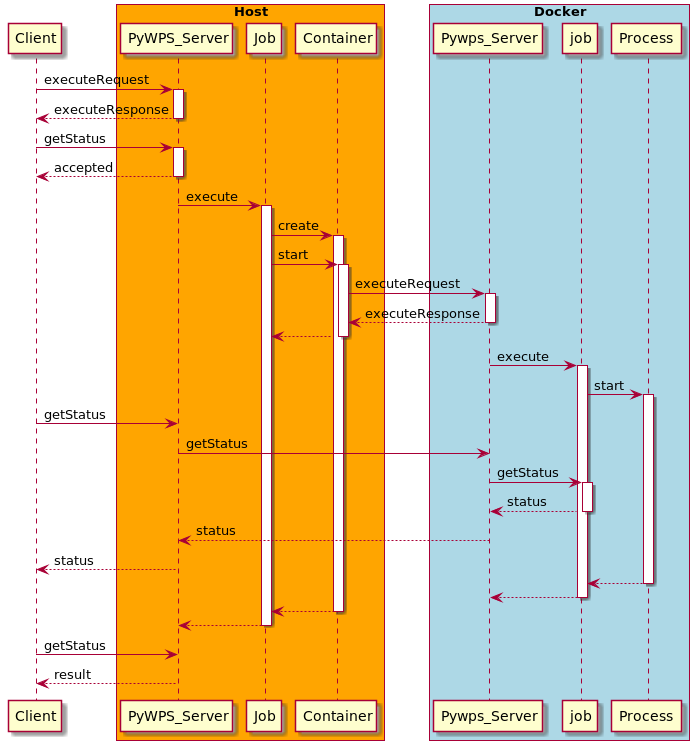
\includegraphics[width=0.9\textwidth]{img/Diag_sequence.png}
\caption{Sequence diagram: Process execution using Docker, source: author}
\label{fig:Diag_sequence}
\end{figure}

\subsection{\textit{Container} class constructor}
\label{sub:Container_init}

%% ML: opravit preteceni textu
%% AL: preteceni opraveno
\textit{Container} class is initialized with standard Python method
\textit{\_\_init\_\_()}. As an inheritor of \textit{Processing} class,
at first the parent constructor \textit{super().\_\_init\_\_()} is called. Follows description of methods
which are called inside the constructor method.

\bigskip
\begin{lstlisting}[basicstyle=\small,caption={\textit{Container} class constructor},label={lst:Container_constructor}]
def __init__(self, process, wps_request, wps_response):
    super().__init__(process, wps_request, wps_response)
    self.port = self._assign_port()
    self.client = docker.from_env()
    self.cntnr = self._create()
\end{lstlisting}

\subsubsection{\textit{Container.\_assign\_port()}}
The method returns the number of available port. The port is chosen from range <\textit{port\_min},
\textit{port\_max}> which are both configurable values. If no port from the range is available, the method returns
\textit{NoAvailablePortException}. Schema of ports assignment to each container is in Fig. \ref{fig:Diag_port}.

\subsubsection{\textit{docker.from\_env()}} The \textit{docker} is a Python library for the Docker Engine API. \textit{from\_env} method
returns an instance of \textit{DockerClient} class which is a client to communicate with the Docker daemon. The returned client is
configured from the same variables as the Docker command-line client.

\subsubsection{\textit{Container.\_create()}} The \textit{\_create} method reads following values at the beginning:
\begin{itemize}
\item \textit{cntnr\_img} - Name of the image the container will be created from. The name of the image must be the same as the tag
set by the \textit{-t} parameter in \textit{docker build} command when the image is built from Dockerfile.

\bigskip
\begin{lstlisting}[basicstyle=\small,caption={Docker build command}]
docker build -t image_name /path/to/dockerfile
\end{lstlisting}

\item \textit{prcs\_inp\_dir} - Path to process workdir from \textit{self.job.wps\_response.process.workdir}. It is a directory where the
inputs for the process are stored.
\item \textit{prcs\_out\_dir} - Path to server output directory where all outputs are stored. The path is taken from \textit{outputpath}
parameter of section \textit{server} in the configuration file.
\item \textit{dckr\_inp\_dir} - Path to input data directory of WPS instance running inside Docker container. It is taken from 
\textit{dckr\_inp\_dir} of \textit{processing} section.
\item \textit{dckr\_out\_dir} - Path to output directory of WPS instance running inside the container. It is taken from 
\textit{dckr\_out\_dir} of \textit{processing} section.
\end{itemize}

The method returns an instance of \textit{Container} class from \textit{docker} module. The container is created by
\textit{self.client.containers.create()} method. 

The method takes optional parameter \textit{ports}. It is a dictionary
that defines ports to bind inside the container. The keys of the
dictionary are the ports to bind inside the container (port 5000
inside \textit{Container 1} and \textit{Container 2} at
Fig. \ref{fig:Diag_port}). The values of the dictionary are the
corresponding ports to open on the host (port 5050 for \textit{Job1},
port 5051 for \textit{Job2} at Fig. \ref{fig:Diag_port}).

\begin{figure}[h!]
\centering
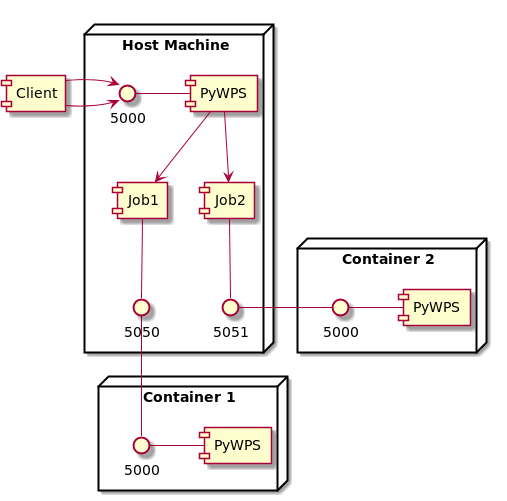
\includegraphics[width=0.55\textwidth]{img/Diag_ports.png}
\caption{Ports assignment schema, source: author}
\label{fig:Diag_port}
\end{figure}

Another optional parameter is \textit{volumes}. It is a dictionary 
to configure volumes mounted inside the container. The key is the host path and the value is a dictionary with the keys: \textit{bind}
- the path to mount the volume inside the container, and \textit{mode} - either \textit{rw} to mount the volume read/write, or 
\textit{ro} to mount it read-only.

%% ML: zdroj
%% AL: tohle predpokladam patri k tomu obrazku o par radku vyse
%% k listingu zdroj snad davat nemusim
%% ML: je to tak
\bigskip
\begin{lstlisting}[basicstyle=\small,caption={\textit{create()} method}]
self.client.containers.create(cntnr_img, detach=True,
ports={"5000/tcp": self.port}, 
volumes={prcs_out_dir: {'bind': dckr_out_dir, 'mode': 'rw'},
         prcs_inp_dir: {'bind': dckr_inp_dir, 'mode': 'ro'}})
\end{lstlisting}

Every container created with defined parameters \textit{volumes} and
\textit{ports} will have output directory on the host mounted into the
container output directory as well as the process workdir at host
machine mounted into container directory with data. Therefore, all
inputs downloaded to process workdir will be available for the
container and all outputs produced after process execution will be
%% ML: Shown?
%% ML: asi nekde zapadlo?
stored at host machine output directory. Displayed in
Fig. \ref{fig:Diag_mount}.

%% ML: zdroj
%% AL: ok
\begin{figure}[h!]
\centering
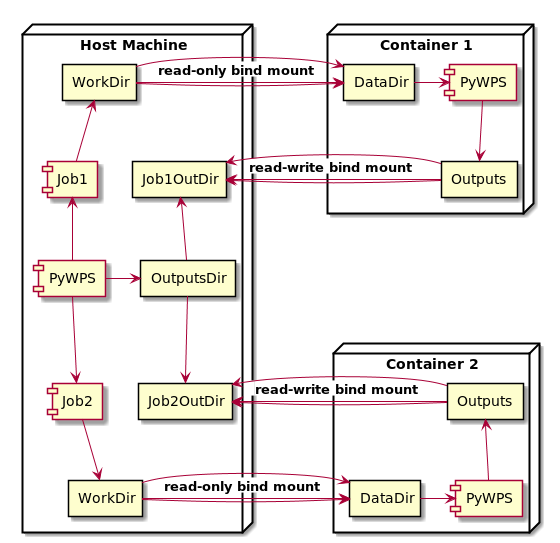
\includegraphics[width=0.65\textwidth]{img/Diag_mount.png}
\caption{Schema of mounting directories, source: author}
\label{fig:Diag_mount}
\end{figure}

%% ML: cela kapitola 9.2 neni uplne ctiva a prehledna (mozna by pomohl
%% opet nejaky diagram), zkus to jeste jednou projit, na velke upravy
%% ale neni cas

%% AL: pridal jsem obrazek, ktery snad trochu pomuze
\subsection{\textit{Container.start()} method}
When a container is created the \textit{start()} method is called and the container is started.
In the time of finishing this thesis the method looks like at Lst.\ref{lst:Container_start}. In the current state is used the method
\textit{\_dirty\_clean()}. It assures that the container is removed after the successful execution, temporary workdir is cleaned and it also 
updates the process status in the database. Unfortunately, it causes that the process runs synchronously. To solve this problem is one of the future goals. The schema of \textit{Container.start()} method is in Fig. \ref{fig:DiagWPSExecute}

%% ML: pokud bys mel ukazku kodu ocislovanou, mohl bys cisla radku
%% pouzivat jako referenci v dalsim textu
%% AL: zkousel jsem to pomoci \lstset, ale cisla radku se vykreslovala 
%% na zacatek/konec radku, ale mimo zarovnani a nevypadalo to moc dobre
%% ML: jj, zakladni formatovani vypisuje radky mimo odstavec, to je OK
%%\lstset{
%%  numbers=right,
%%  numbersep=1pt
%%}

\newpage
\begin{lstlisting}[basicstyle=\small,caption={\textit{Container.create()} method},label={lst:Container_start}]
def start(self):
    self.cntnr.start()
    time.sleep(0.5)
    self._execute()
    self._parse_status()
    self._dirty_clean()
\end{lstlisting}

\subsubsection{\textit{docker.container.start()}}
\textit{start()} method of \textit{Container} class from Python module \textit{docker}. The method is similar to \textit{docker start} command. 
It starts the Docker container. Then the method \textit{time.sleep()} is called to wait half a second after which the container is ready to 
use.

\subsubsection{\textit{Container.\_execute()}}
\label{sub:Container_execute}
\textit{\_execute()} method handles forwarding execution from server
to container. For sending request to container \textit{OWSLib}
%% ML: misto poznamky pod carou uved odkaz na kapitolu
%% AL: predelano
library (Sec. \ref{sub:owslib}) is used.

\paragraph{OWSLib} is a Python package for client programming with OGC web services interface standards. However before it was possible
to use this package it was necessary to fix a bug in the \textit{wps} module. The bug caused outputs in the Execute response, which
were referenced as web-accesible resource, not to be parsed because of wrong handling with \textit{xlink} namespace. The bug-fix diff file 
is available in App. \ref{app:owslib}. 

\begin{lstlisting}[basicstyle=\small,caption={\textit{Container.\_execute()} method},label={lst:Container._execute}]
def _execute(self):
    url_execute = "http://localhost:{}/wps".format(self.port)
    inputs = get_inputs(self.job.wps_request.inputs)
    output = get_output(self.job.wps_request.outputs)
    wps = WPS(url=url_execute, skip_caps=True)
    self.execution = wps.execute(self.job.wps_request.identifier,
                                 inputs=inputs, output=output)
\end{lstlisting}

The method calls \textit{get\_inputs()} that 
returns all inputs transformed into a list of tuples in form \textit{(input\_name, input\_value)}. In case of ComplexData input, the input value is replaced with path to file. It is necessary to transform the inputs into the list of tuples because it is the required form for
\textit{WebProcessingService.execute()} method. Example for demo process \textit{buffer} at Lst. \ref{lst:Container.get_inputs}.

\begin{lstlisting}[basicstyle=\small,caption={\textit{get\_inputs} return value},label={lst:Container.get_inputs}]
the_inputs = [('poly_in', 'file:///pywps-flask/data/point.gml'),
              ('buffer', '1.0')]
the_outputs = [('buff_out', 'true')]
\end{lstlisting}

Then the method calls \textit{get\_outputs()} that returns list of tuples in form \textit{(output\_name, asReference\_attr\_value)}. It is 
necessary to transform the outputs into the list of tuples because it is the required form for \textit{WebProcessingService.execute()} method. 

\textit{WebProcessingService} object from OWSLib package is responsible for sending request to container. Its constructor takes URL of the
WPS server running inside container. Container URL varies depending on the port assigned to the container. Then the \textit{WPSExecution}
object is assigned to the \textit{Container} instance. The WPS\-Execution object is returned from \textit{WebProcessingService.execute()} 
method that takes as inputs process identifier, list of inputs from \textit{get\_inputs()} and outputs from \textit{get\_outputs()}.

\subsubsection{\textit{Container.\_parse\_status()}}
The method takes path to status location from \textit{WPSExecution.statusLocation} and copies it to \textit{Job.process.status\_url}.
Then the \textit{WPSReponse} object is updated by \textit{Job.wps\_response.update\_status()} with \textit{WPSExecution.statusMessage}.
It means the \textit{WPSResponse} object at host machine WPS server adopts \textit{statusMessage} and path to \textit{statusLocation}
from \textit{WPSExecution} object that handles the process execution inside the container. The process execution inside the container
updates its status into the file that is located in container output directory. This directory is shared with WPS server at host machine
so it is available even for the client.

\subsubsection{\textit{Container.\_dirty\_clean()}}
The method cares about stopping and removing Docker container, removing job workdir and original status XML. This method prevents from
accumulation of running Docker containers and temporary files in workdir directory. On the other hand there is missing functionality
for the process managment in database. In the current state when using Docker, the processes on the server are not ended even though
the result is already returned from the container. These pseudo-running processes accumulate on the server and some other processes
can be rejected because the limit of maximal running  processes is reached. This must be solved in the future.

\begin{lstlisting}[basicstyle=\small,caption={\textit{get\_inputs} return value},label={lst:Container.get_inputs}]
def _dirty_clean(self):
    time.sleep(1)
    self.cntnr.stop()
    self.cntnr.remove()
    self.job.process.clean()
    os.remove(self.job.process.status_location)
\end{lstlisting}

\textit{time.sleep(1)} is called to wait one second so the running process execution inside the container can be finished. The parameter
1 second is hardcoded and serves just now when the development is not done. \textit{stop()} and \textit{remove()} methods of class 
\textit{Container} from \textit{docker} module are similar to docker commands \textit{docker stop container\_id} and 
\textit{docker rm container\_id}.

\textit{Job.process.clean()} remove the job workdir so the temporary files do not cumulate at the server. \textit{os.remove()} deletes
the original status XML since the status XML from the container was sent back to the client.

\begin{figure}[h!]
\centering
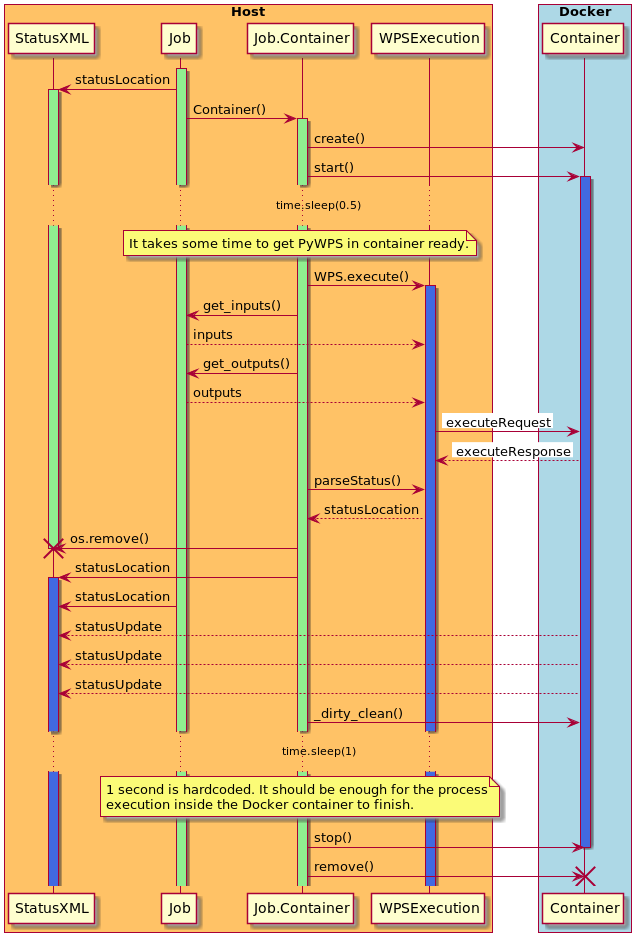
\includegraphics[width=0.7\textwidth]{img/Diag_WPSExecute.png}
\caption{Schema of \textit{WPSExecution}, source: author}
\label{fig:DiagWPSExecute}
\end{figure}


\newpage
\necislovana{Závěr}
\todo[inline]{Dopsat zaver}

\newpage
\necislovana{Seznam použitých zkratek}

\begin{tabular}{ll}
\textbf{API}& Application Programming Interface\\
\textbf{CGAL}& Computational Geometry Algorithms Library\\
\textbf{GDAL}& Geospatial Data Abstraction Library\\
\textbf{GIS}& Geographic Information System\\
\textbf{HPC}& High Performance Compute\\
\textbf{KVP}& Key Value Pair\\
\textbf{OGC}& Open Geospatial Consortium\\
\textbf{PID}& Process identifier \\
\textbf{SOAP}& Simple Object Access Protocol \\
\textbf{URL}& Uniform Resource Locator\\
\textbf{VM}& Virtual Machine\\
\textbf{VMM}& Virtual Machine Monitor\\
\textbf{WPS}& Web Processing Service\\
\textbf{WMS}& Web Map Service\\
\textbf{WFS}& Web Feature Service\\
\textbf{WCS}& Web Coverage Service\\
\textbf{XML}& eXtensible Markup Language\\
\end{tabular}

\newpage
\begin{thebibliography}{99}
\label{Bibliography}
\bibitem{OGC_news}
Mark Reichardt \textit{OGC Newsletter - October 2004, OGC document number 04-043} [online].
URL: \textless\url{http://www.opengeospatial.org/pressroom/newsletters/200410}\textgreater

\bibitem{WPS_experiment}
Sam Bacharach \textit{OGC announces Web Processing Services Interoperability Experiment} [online].
URL: \textless\url{http://www.opengeospatial.org/pressroom/pressreleases/414}\textgreater

\bibitem{WPS_first}
Open Geospatial Consortium Inc. \textit{OpenGIS ® Web Processing Service, OGC document number 05-007r4, ver. 0.4.0} [online].
URL: \textless\url{https://portal.opengeospatial.org/files/?artifact_id=13149&version=1&format=doc}\textgreater

\bibitem{OGC}
Open Geospatil Consorcium \textit{OGC websites} [online].
URL: \textless\url{http://www.opengeospatial.org/}\textgreater

\bibitem{OGC_history}
Open Geospatil Consorcium \textit{OGC History (detailed)} [online].
URL: \textless\url{http://www.opengeospatial.org/ogc/historylong}\textgreater

\bibitem{WPS_standart_1.0}
http://www.opengeospatial.org/pressroom/newsletters/200410

\bibitem{WPS_second}
Open Geospatial Consortium \textit{OGC® WPS 2.0 Interface Standard Corrigendum 1, OGC document number 06-121r3} [online].
URL: \textless\url{https://portal.opengeospatial.org/files/?artifact_id=13149&version=1&format=doc}\textgreater

\bibitem{OGC_common}
Open Geospatial Consortium Inc. \textit{OGC Web Services Common Specification, OGC document number 14-065} [online].
URL: \textless\url{https://portal.opengeospatial.org/files/?artifact_id=20040}\textgreater

\bibitem{deegree_docs}
deegree devs \textit{deegree documentation} [online].
URL: \textless\url{http://download.deegree.org/documentation/3.3.20/html/}\textgreater

\bibitem{GS_docs}
GeoServer devs \textit{GeoServer documentation} [online].
URL: \textless\url{http://docs.geoserver.org/}\textgreater

\bibitem{ZOO_docs}
ZOO-Project devs \textit{ZOO-Project documentation} [online].
URL: \textless\url{http://zoo-project.org/docs}\textgreater

\bibitem{AG_docs}
Esri \textit{Tuning and configuring services} [online].
URL: \textless\url{http://server.arcgis.com/en/server/latest/publish-services/linux/tuning-and-configuring-services.htm}\textgreater

\bibitem{Docker_docs}
Docker \textit{Docker documentation} [online].
URL: \textless\url{https://docs.docker.com/}\textgreater

\bibitem{PyWPS_paper}
Jáchym Čepický, Luís Moreira de Sousa \textit{New implementation of OGC Web Processing Service in Python programming language.} [online].
URL: \textless\url{https://www.int-arch-photogramm-remote-sens-spatial-inf-sci.net/XLI-B7/927/2016/isprs-archives-XLI-B7-927-2016.pdf}\textgreater

\bibitem{PyWPS_presentation}
Jorge de Jesus, Luca Casagrande, Jáchym Čepický \textit{PyWPS a tutorial for beginners and developers} [online].
URL: \textless\url{https://www.slideshare.net/JorgeMendesdeJesus/pywps-a-tutorial-for-beginners-and-developers}\textgreater

\bibitem{PyWPS_web}
PyWPS developers \textit{PyWPS History} [online].
URL: \textless\url{http://pywps.org/history/}\textgreater

\bibitem{PyWPS_docs}
PyWPS developers \textit{PyWPS documentation} [online].
URL: \textless\url{http://pywps.readthedocs.io/}\textgreater

\bibitem{PyDev_ML}
Victor Stinner \textit{The pysandbox project is broken} [online].
URL: \textless\url{https://lwn.net/Articles/574323/}\textgreater

\bibitem{Korea}
Victor Stinner \textit{Linkage of OGC WPS 2.0 to the e-Government Standard Framework in Korea: An Implementation Case for Geo-Spatial Image Processing} [online].
URL: \textless\url{http://www.mdpi.com/2220-9964/6/1/25/pdf}\textgreater
\end{thebibliography}

\newpage
\part{Appendix}

\appendix
\newpage
\section{Execute request example}
\label{app:ExecuteRequest}
\begin{lstlisting}[basicstyle=\small,caption={Execute request example}]
<?xml version="1.0" encoding="UTF-8" standalone="yes"?>
<wps:Execute service="WPS" version="1.0.0" xmlns:wps="http://www.opengis.net/wps/1.0.0" xmlns:ows="http://www.opengis.net/ows/1.1" xmlns:xlink="http://www.w3.org/1999/xlink" xmlns:xsi="http://www.w3.org/2001/XMLSchema-instance" xsi:schemaLocation="http://www.opengis.net/wps/1.0.0 ../wpsExecute_request.xsd">
 <ows:Identifier>buffer</ows:Identifier>
 <wps:DataInputs>
  <wps:Input>
   <ows:Identifier>poly_in</ows:Identifier>
   <wps:Reference xlink:href="http://localhost:5000/static/data/point.gml" />
  </wps:Input>
  <wps:Input>
   <ows:Identifier>buffer</ows:Identifier>
   <wps:Data>
    <wps:LiteralData>1</wps:LiteralData>
   </wps:Data>
  </wps:Input>
 </wps:DataInputs>
 <wps:ResponseForm>
  <wps:ResponseDocument status="true" storeExecuteRsponse="true">
   <wps:Output asReference="true">
    <ows:Identifier>buff_out</ows:Identifier>
   </wps:Output>
  </wps:ResponseDocument>
 </wps:ResponseForm>
</wps:Execute>
\end{lstlisting}

\newpage
\section{Execute response example (async mode)}
\label{app:ExecuteResponse}
\begin{lstlisting}[basicstyle=\small,caption={Execute response example (async mode)}]
<!-- PyWPS 4.0.0 -->
<wps:ExecuteResponse xmlns:gml="http://www.opengis.net/gml" 
  xmlns:ows="http://www.opengis.net/ows/1.1" 
  xmlns:wps="http://www.opengis.net/wps/1.0.0" 
  xmlns:xlink="http://www.w3.org/1999/xlink" 
  xmlns:xsi="http://www.w3.org/2001/XMLSchema-instance" 
  xsi:schemaLocation="http://www.opengis.net/wps/1.0.0 
  http://schemas.opengis.net/wps/1.0.0/wpsExecute_response.xsd" 
  service="WPS" version="1.0.0" xml:lang="en-US" 
  serviceInstance="http://localhost:5000/wps?service=WPS&request=
  GetCapabilities" 
  statusLocation="http://localhost:5000/outputs/ce57acbe-f1f3-11
  e7-ad2a-0242ac110003.xml">
 <wps:Process wps:processVersion="0.1">
  <ows:Identifier>buffer</ows:Identifier>
  <ows:Title>GDAL Buffer process</ows:Title>
  <ows:Abstract>
   The process returns buffers around the input features,
   using the GDAL library
  </ows:Abstract>
 </wps:Process>
 <wps:Status creationTime="2018-01-05T09:38:41Z">
  <wps:ProcessAccepted>
   PyWPS Process buffer accepted
  </wps:ProcessAccepted>
 </wps:Status>
</wps:ExecuteResponse
\end{lstlisting}

\newpage
\section{Status XML example with referenced output}
\label{app:status_reference}
\begin{lstlisting}[basicstyle=\small,caption={Status XML example}]
<wps:ExecuteResponse
  xsi:schemaLocation="http://www.opengis.net/wps/1.0.0 
  http://schemas.opengis.net/wps/1.0.0/wpsExecute_response.xsd" 
  service="WPS" version="1.0.0" xml:lang="en-US"
  serviceInstance="http://localhost:5000/wps?service=WPS&request=
  GetCapabilities" 
  statusLocation="http://localhost:5000/outputs/ce57acbe-f1f3-11
  e7-ad2a-0242ac110003.xml">
 <wps:Process wps:processVersion="0.1">
  <ows:Identifier>buffer</ows:Identifier>
  <ows:Title>GDAL Buffer process</ows:Title>
  <ows:Abstract>
   The process returns buffers around the input features,
   using the GDAL library
  </ows:Abstract>
 </wps:Process>
 <wps:Status creationTime="2018-01-05T08:38:30Z">
  <wps:ProcessSucceeded>
   PyWPS Process GDAL Buffer process finished
  </wps:ProcessSucceeded>
 </wps:Status>
 <wps:ProcessOutputs>
  <wps:Output>
   <ows:Identifier>buff_out</ows:Identifier>
   <ows:Title>Buffered file</ows:Title>
   <wps:Reference xlink:href="http://localhost:5000/outputs/ce57acbe-f1f3-11e7-ad2a-0242ac110003/point_buffer_42rkmvt1.gml" mimeType="application/gml+xml"/>
  </wps:Output>
 </wps:ProcessOutputs>
</wps:ExecuteResponse>
\end{lstlisting}

\section{Status XML example with inline output}
\label{app:status_inline}
\begin{lstlisting}[basicstyle=\small,caption={Status XML example}]
<wps:ExecuteResponse
  xsi:schemaLocation="http://www.opengis.net/wps/1.0.0 
  http://schemas.opengis.net/wps/1.0.0/wpsExecute_response.xsd" 
  service="WPS" version="1.0.0" xml:lang="en-US" 
  serviceInstance="http://localhost:5000/wps?service=WPS&request=
  GetCapabilities" 
  statusLocation="http://localhost:5000/outputs/1cd3e506-f1f7-11
  e7-8546-0242ac110003.xml">
 <wps:Process wps:processVersion="0.1">
  <ows:Identifier>buffer</ows:Identifier>
  <ows:Title>GDAL Buffer process</ows:Title>
  <ows:Abstract>
   The process returns buffers around the input features,
   using the GDAL library
  </ows:Abstract>
 </wps:Process>
 <wps:Status creationTime="2018-01-05T09:02:10Z">
  <wps:ProcessSucceeded>
   PyWPS Process GDAL Buffer process finished
  </wps:ProcessSucceeded>
 </wps:Status>
 <wps:ProcessOutputs>
  <wps:Output>
   <ows:Identifier>buff_out</ows:Identifier>
   <ows:Title>Buffered file</ows:Title>
   <wps:Data>
    <wps:ComplexData mimeType="application/gml+xml">
     <ogr:FeatureCollection xmlns:ogr="http://ogr.maptools.org/" 
       xsi:schemaLocation="http://schemas.opengis.net/gml/2.1.2/
       feature.xsd">
      <gml:boundedBy>
       <gml:Box>
        <gml:coord>
         <gml:X>-0.9514645979959721</gml:X>
         <gml:Y>-0.986306232731747</gml:Y>
        </gml:coord>
        <gml:coord>
         <gml:X>1.048535402004028</gml:X>
         <gml:Y>1.013693767268253</gml:Y>
        </gml:coord>
       </gml:Box>
      </gml:boundedBy>
      <gml:featureMember>
      <ogr:point_buffer fid="point_buffer.0">
       <ogr:geometryProperty>
        <gml:Polygon>
         <gml:outerBoundaryIs>
          <gml:LinearRing>
           <gml:coordinates>1.04853540200403,0.013693767268253 
           1.0471649367586,-0.038642188974691  0.857552396378976,
           -0.57409148502422 0.825681363460999,-0.615626623781584 
           0.791680227481423,-0.655436839090605 0.75564218319056,
           -0.852331636516187 -0.496103633010996,-0.8249768006773
           -0.539249850288442,-0.795323227106697 -0.580784989006,
           -0.763452194188721 -0.620595204354827,-0.7294510582044
           </gml:LinearRing>
          </gml:outerBoundaryIs>
         </gml:Polygon>
        </ogr:geometryProperty>
       </ogr:point_buffer>
      </gml:featureMember>
     </ogr:FeatureCollection>
    </wps:ComplexData>
   </wps:Data>
  </wps:Output>
 </wps:ProcessOutputs>
</wps:ExecuteResponse>
\end{lstlisting}

\newpage
\section{Dockerfile}
\label{app:dockerfile}
\begin{lstlisting}[basicstyle=\small,caption={Dockerfile example}]
FROM alpine:latest
MAINTAINER Jorge S. Mendes de Jesus <jorge.dejesus@geocat.net>

ENV GDAL_VERSION 2.2.0
ENV XERCES_VERSION 3.2.0

RUN apk add --no-cache \
	git \
	gcc \
	bash \
	openssh \
	musl-dev  \
	python3 \
	python3-dev \
	libxml2-dev  \
	libxslt-dev \
	linux-headers \
	expat \
	expat-dev


RUN apk --update --no-cache add g++ libstdc++ make swig

# Xerces
RUN wget http://www.apache.org/dist/xerces/c/3/sources/xerces-c-${XERCES_VERSION}.tar.gz -O /tmp/xerces-c-${XERCES_VERSION}.tar.gz && \
    tar xvf /tmp/xerces-c-${XERCES_VERSION}.tar.gz -C /tmp && \
    cd /tmp/xerces-c-${XERCES_VERSION} && \
    ./configure --prefix=/opt/xerces && \
    make -j 4 && \
    make install

# Geos
RUN apk add --no-cache \
    --repository http://dl-cdn.alpinelinux.org/alpine/edge/testing \
    geos \
    geos-dev

# Install GDAL
RUN wget http://download.osgeo.org/gdal/${GDAL_VERSION}/gdal-${GDAL_VERSION}.tar.gz -O /tmp/gdal.tar.gz && \
	tar xzf /tmp/gdal.tar.gz -C /tmp && \
	cd /tmp/gdal-${GDAL_VERSION} && \
	CFLAGS="-g -Wall" LDFLAGS="-s" ./configure --with-expat=yes --with-xerces=/opt/xerces --with-geos=yes \
	&& make -j 4 && make install

RUN cd /tmp/gdal-${GDAL_VERSION}/swig/python \
	&& python3 setup.py build \
	&& python3 setup.py install

RUN git clone https://github.com/lazaa32/pywps-flask.git

WORKDIR /pywps-flask
RUN pip3 install -r requirements.txt


EXPOSE 5000
ENTRYPOINT ["/usr/bin/python3", "demo.py","-a"]

#docker build -t pywps-flask .
#docker run -p 5000:5000 pywps-flask
#http://localhost:5000/wps?request=GetCapabilities&service=WPS
#http://localhost:5000/wps?request=DescribeProcess&service=WPS&identifier=all&version=1.0.0
\end{lstlisting}

\newpage
\section{OWSLib diff file}
\label{app:owslib}
\begin{lstlisting}[basicstyle=\small,caption={OWSLib diff file}]
diff --git a/owslib/wps.py b/owslib/wps.py
index c16e288..ce86f93 100644
--- a/owslib/wps.py
+++ b/owslib/wps.py
@@ -1117,13 +1117,15 @@ class Output(InputOutput):
 
   # extract wps namespace from outputElement itself
   wpsns = getNamespace(outputElement)
+  # extract xlink namespace
+  xlins =outputElement.nsmap['xlink']
 
   # <ns:Reference encoding="UTF-8" mimeType="text/csv"
   # href="http://cida.usgs.gov/climate/gdp/process/RetrieveResultServlet?id=1318528582026OUTPUT.601bb3d0-547f-4eab-8642-7c7d2834459e"
   # />
   referenceElement = outputElement.find(nspath('Reference', ns=wpsns))
   if referenceElement is not None:
-      self.reference = referenceElement.get('href')
+      self.reference = referenceElement.get('{{{}}}href'.format(xlins))
       self.mimeType = referenceElement.get('mimeType')
 
   # <LiteralOutput>
\end{lstlisting}

\newpage
\section{pywps-demo diff file}
\label{app:pywps-demo}
\begin{lstlisting}[basicstyle=\small,caption={pywps-demo diff file}]
diff --git a/pywps.cfg b/pywps.cfg
index a1ed125..f6e3981 100644
--- a/pywps.cfg
+++ b/pywps.cfg
@@ -28,14 +28,25 @@ maxrequestsize=3mb
 url=http://localhost:5000/wps
 outputurl=http://localhost:5000/outputs/
 outputpath=outputs
-workdir=/tmp
+workdir=workdir
+wd_inp_subdir=inputs
+wd_out_subdir=outputs
 maxprocesses=10
-parallelprocesses=2
+parallelprocesses=6
+
+[processing]
+mode=multiprocessing
+port_min=5050
+port_max=5070
+docker_img=pywps_container
+dckr_inp_dir=/pywps-flask/data
+dckr_out_dir=/pywps-flask/outputs
 
 [logging]
 level=INFO
 file=logs/pywps.log
 database=sqlite:///logs/pywps-logs.sqlite3
+format=%(asctime)s] [%(levelname)s] file=%(pathname)s line=%(lineno)s module=%(module)s function=%(funcName)s %(message)s
 
 
 [grass]
diff --git a/requirements.txt b/requirements.txt
index f9884fd..327038c 100644
--- a/requirements.txt
+++ b/requirements.txt
@@ -1,12 +1,13 @@
-Flask==0.10.1
-Jinja2==2.7.3
-jsonschema==2.5.1
-lxml==3.3.3
-OWSLib==0.11.2
-pyproj==1.9.5.1
-requests==2.11.1
-Shapely==1.5.7
-Werkzeug==0.10.4
-SQLAlchemy==1.0.15
-psutil==4.3.1
--e git+https://github.com/geopython/pywps.git@master#egg=pywps-master
+Flask
+Jinja2
+jsonschema
+lxml
+OWSLib
+pyproj
+requests
+Shapely
+Werkzeug
+SQLAlchemy
+psutil
+docker
+-e git+https://github.com/lazaa32/pywps.git@develop#egg=pywps-develop

diff --git a/setup.py b/setup.py
index d4a5f6a..7c92362 100644
--- a/setup.py
+++ b/setup.py
@@ -50,7 +50,7 @@ config = {
     'license': 'MIT',
     'platforms': 'all',
     'url': 'http://pywps.org',
-    'download_url': 'https://github.com/geopython/pywps-flask',
+    'download_url': 'https://github.com/lazaa32/pywps-flask',
     'author_email': 'luis.a.de.sousa@gmail.com',
     'maintainer': 'Luis de Sousa',
     'maintainer_email': 'luis.de.sousa@protonmail.ch',
@@ -67,7 +67,7 @@ config = {
     'version': VERSION,
     'install_requires': INSTALL_REQUIRES,
     'dependency_links': [
-        'git+https://github.com/geopython/pywps.git@pywps-'+VERSION+'#egg=pywps-'+VERSION
+        'git+https://github.com/lazaa32/pywps.git@pywps-'+VERSION+'#egg=pywps-'+VERSION
      ],
     'packages': ['processes', 'tests'],
     'scripts': ['demo.py'],
\end{lstlisting}

\newpage
\section{pywps diff file}
\begin{lstlisting}[basicstyle=\small,caption={pywps diff file}]
diff --git a/pywps/exceptions.py b/pywps/exceptions.py
index 8483911..e0e1c57 100644
--- a/pywps/exceptions.py
+++ b/pywps/exceptions.py
@@ -150,3 +150,10 @@ class SchedulerNotAvailable(NoApplicableCode):
     """Job scheduler not available exception implementation
     """
     code = 400
+
+
+class NoAvailablePortException(NoApplicableCode):
+    """
+    No port available for new docker.
+    """
+    code = 400
diff --git a/pywps/processing/__init__.py b/pywps/processing/__init__.py
index 03bf0af..63816e1 100644
--- a/pywps/processing/__init__.py
+++ b/pywps/processing/__init__.py
@@ -7,6 +7,7 @@
 import pywps.configuration as config
 from pywps.processing.basic import MultiProcessing
 from pywps.processing.scheduler import Scheduler
+from pywps.processing.container import Container
 # api only
 from pywps.processing.basic import Processing  # noqa: F401
 from pywps.processing.job import Job  # noqa: F401
@@ -16,6 +17,7 @@ LOGGER = logging.getLogger("PYWPS")
 
 MULTIPROCESSING = 'multiprocessing'
 SCHEDULER = 'scheduler'
+DOCKER = 'docker'
 DEFAULT = MULTIPROCESSING
 
 
@@ -30,6 +32,8 @@ def Process(process, wps_request, wps_response):
     LOGGER.info("Processing mode: %s", mode)
     if mode == SCHEDULER:
         process = Scheduler(process, wps_request, wps_response)
+    elif mode == DOCKER:
+        process = Container(process, wps_request, wps_response)
     else:
         process = MultiProcessing(process, wps_request, wps_response)
     return process
diff --git a/pywps/processing/container.py b/pywps/processing/container.py
new file mode 100644
index 0000000..8f5151e
--- /dev/null
+++ b/pywps/processing/container.py
@@ -0,0 +1,155 @@
+##################################################################
+# Copyright 2016 OSGeo Foundation,                               #
+# represented by PyWPS Project Steering Committee,               #
+# licensed under MIT, Please consult LICENSE.txt for details     #
+##################################################################
+
+import os
+import shutil
+import pywps.configuration as config
+from pywps.processing.basic import Processing
+
+from owslib.wps import WebProcessingService as WPS
+from pywps.response.status import STATUS
+from pywps.exceptions import NoAvailablePortException
+import docker
+import socket
+import time
+
+from pywps.inout.basic import LiteralInput, ComplexInput, BBoxInput
+import owslib
+from pywps.dblog import update_response
+
+
+import logging
+LOGGER = logging.getLogger("PYWPS")
+
+
+class ClientError:
+    pass
+
+
+class Container(Processing):
+    def __init__(self, process, wps_request, wps_response):
+        super().__init__(process, wps_request, wps_response)
+        self.port = self._assign_port()
+        self.client = docker.from_env()
+        self.cntnr = self._create()
+
+    def _create(self):
+        cntnr_img = config.get_config_value("processing", "docker_img")
+        prcs_inp_dir = self.job.wps_response.process.workdir
+        prcs_out_dir = config.get_config_value("server", "outputpath")
+        dckr_inp_dir = config.get_config_value("processing", "dckr_inp_dir")
+        dckr_out_dir = config.get_config_value("processing", "dckr_out_dir")
+        container = self.client.containers.create(cntnr_img, ports={"5000/tcp": self.port}, detach=True,
+                                                  volumes={
+                                                  prcs_out_dir: {'bind': dckr_out_dir, 'mode': 'rw'},
+                                                  prcs_inp_dir: {'bind': dckr_inp_dir, 'mode': 'ro'}
+                                                  })
+        return container
+
+    def _assign_port(self):
+        port_min = int(config.get_config_value("processing", "port_min"))
+        port_max = int(config.get_config_value("processing", "port_max"))
+        for port in range(port_min, port_max):
+            sock = socket.socket(socket.AF_INET, socket.SOCK_STREAM)
+            res = sock.connect_ex(('127.0.0.1', port))
+            # TODO find better solution for errno
+            if res != 0:
+                return port
+        raise NoAvailablePortException("No port from range {}-{} available.".format(port_min, port_max))
+
+    def start(self):
+        self.cntnr.start()
+        # TODO it takes some time to start the container
+        time.sleep(0.5)
+        self._execute()
+        self._parse_status()
+        self._dirty_clean()
+
+    def stop(self):
+        self.cntnr.stop()
+
+    def cancel(self):
+        self.cntnr.kill()
+
+    def pause(self):
+        self.cntnr.pause()
+
+    def unpause(self):
+        self.cntnr.unpause()
+
+    def _execute(self):
+        url_execute = "http://localhost:{}/wps".format(self.port)
+        inputs = get_inputs(self.job.wps_request.inputs)
+        output = get_output(self.job.wps_request.outputs)
+        wps = WPS(url=url_execute, skip_caps=True)
+        self.execution = wps.execute(self.job.wps_request.identifier, inputs=inputs, output=output)
+
+    # Obsolete function when docker was called in synchro mode
+    def _parse_outputs(self):
+        for output in self.execution.processOutputs:
+            # TODO what if len(data) > 1 ??
+            if output.data:
+                self.job.wps_response.outputs[output.identifier].data = output.data[0]
+            if output.reference:
+                rp = output.reference[output.reference.index('outputs/'):]
+                self.job.wps_response.outputs[output.identifier].file = rp
+
+        self.job.wps_response.update_status('PyWPS process {} finished'.format(self.job.process.identifier),
+                                            status_percentage=100, status=STATUS.DONE_STATUS)
+
+    def _parse_status(self):
+        self.job.process.status_url = self.execution.statusLocation
+        self.job.wps_response.update_status(message=self.execution.statusMessage)
+
+    def _dirty_clean(self):
+        # TODO wait then stop&remove container
+        time.sleep(1)
+        self.cntnr.stop()
+        self.cntnr.remove()
+        self.job.process.clean()
+        os.remove(self.job.process.status_location)
+        # update_response(self.job.wps_response.uuid, self.job.wps_response)
+        # self.job.wps_response.update_status('PyWPS Process {} finished'.format(self.job.process.title), 100,
+        #                                     STATUS.DONE_STATUS, clean=self.job.process.async)
+
+
+def get_inputs(job_inputs):
+    """
+    Return all inputs in [(input_name1, input_value1), (input_name2, input_value2)]
+    Return value can be used for WPS.execute method.
+    :return: input values
+    :rtype:list of tuples
+    """
+    the_inputs = []
+    for key in job_inputs.keys():
+        inp = job_inputs[key][0]
+        if isinstance(inp, LiteralInput):
+            # TODO use inp.source or inp.data?
+            ows_inp = str(job_inputs[key][0].source)
+        elif isinstance(inp, ComplexInput):
+            fp = os.path.basename(job_inputs[key][0].file)
+            dckr_inp_dir = config.get_config_value('processing', 'dckr_inp_dir')
+            ows_inp = owslib.wps.ComplexDataInput("file://" + os.path.join(dckr_inp_dir, fp))
+        elif isinstance(inp, BBoxInput):
+            ows_inp = owslib.wps.BoundingBoxDataInput(job_inputs[key][0].source)
+        else:
+            raise Exception
+        the_inputs.append((key, ows_inp))
+
+    return the_inputs
+
+
+def get_output(job_output):
+    """
+    Return all outputs name
+    Return value can be used for WPS.execute method.
+    :return: output names
+    :rtype:list
+    """
+    the_output = []
+    for key in job_output.keys():
+        the_output.append((key, job_output[key]['asReference']))
+    return the_output
diff --git a/pywps/processing/job.py b/pywps/processing/job.py
index b855599..f7fe2bc 100644
--- a/pywps/processing/job.py
+++ b/pywps/processing/job.py
@@ -38,7 +38,7 @@ class Job(object):
         LOGGER.debug('dump job ...')
         import dill
         filename = tempfile.mkstemp(prefix='job_', suffix='.dump', dir=self.workdir)[1]
-        with open(filename, 'w') as fp:
+        with open(filename, 'wb') as fp:
             dill.dump(self, fp)
             LOGGER.debug("dumped job status to %s", filename)
             return filename
diff --git a/pywps/response/execute.py b/pywps/response/execute.py
index f78cfb0..e994de3 100644
--- a/pywps/response/execute.py
+++ b/pywps/response/execute.py
@@ -15,7 +15,7 @@ from pywps import WPS, OWS
 from pywps.app.basic import xml_response
 from pywps.exceptions import NoApplicableCode
 import pywps.configuration as config
-import pywps.dblog
+from pywps.dblog import update_response
 
 from pywps.response.status import STATUS
 from pywps.response import WPSResponse
@@ -38,6 +38,33 @@ class ExecuteResponse(WPSResponse):
         self.process = kwargs["process"]
         self.outputs = {o.identifier: o for o in self.process.outputs}
 
+    def update_status(self, message=None, status_percentage=None, status=None,
+                      clean=True):
+        """
+        Update status report of currently running process instance
+
+        :param str message: Message you need to share with the client
+        :param int status_percentage: Percent done (number betwen <0-100>)
+        :param pywps.app.WPSResponse.STATUS status: process status - user should usually
+            ommit this parameter
+        """
+
+        if message:
+            self.message = message
+
+        if status:
+            self.status = status
+
+        if status_percentage:
+            self.status_percentage = status_percentage
+
+        # check if storing of the status is requested
+        if self.status >= STATUS.STORE_AND_UPDATE_STATUS:
+            # rebuild the doc and update the status xml file
+            self.doc = self._construct_doc()
+            self.write_response_doc(clean)
+
+        update_response(self.uuid, self)
 
     def write_response_doc(self, clean=True):
         # TODO: check if file/directory is still present, maybe deleted in mean time
\end{lstlisting}

\newpage
\section{Docker extension documentation}
\label{app:docker_ext_docs}
\begin{lstlisting}[basicstyle=\small,caption={Docker extension documentation}]
.. _docker:

Docker Container Extension
==========================

To isolate each process execution it is possible to enable docker extension.

.. note:: The PyWPS process implementations are not changed by using the
  scheduler extension.

First of all install Docker from `website <https://docs.docker.com/engine/installation/linux/docker-ce/ubuntu/>`_.

Clone ``pywps-demo``::

  $ git clone https://github.com/lazaa32/pywps-flask.git

Install demo requirements from ``requirement.txt``. It will download all required packages including
``pywps`` core package::

  $ cd pywps-flask
  $ pip install -r requirements.txt

``pywps`` package was downloaded to ``src`` directory. Let's set the ``PYTHONPATH`` so ``pywps-demo`` knows
where to find::

  $ EXPORT PYTHONPATH=$PYTHONPATH:$PWD/src/pywps-develop

If everything went OK, it should be now possible to run::

  $ python3 demo.py

However the demo still runs without Docker extension. First of all it is necessary to build an image from Dockerfile.
From the image all containers will be created::

  $ cd docker/isolation
  $ docker build -t container .

.. note:: The **-t** flag sets a name and optionally a tag in the **name:tag** format. The name of the image
   will be one of the parameter value in configuration file.
.. warning:: The image build can take up to several tens of minutes since some manual installation run on the
   background.

You can check the image was built by::

  $ docker images

To activate this extension you need to edit the ``pywps.cfg`` configuration file and make the following changes::

  [processing]
  mode=docker
  port_min=5050
  port_max=5070
  docker_img=container
  dckr_inp_dir=/pywps-flask/data
  dckr_out_dir=/pywps-flask/outputs

``mode`` must be set to ``docker``. ``port_min`` and ``port_max`` define the range of ports which can be
assigned to containers. ``docker_img`` must match to name of the image given by -t flag during the image build.

The docker extension is now enabled and every asynchronous request will be executed separately in a Docker
container.
\end{lstlisting}

\newpage
\section{List of tables and figures}
\listoftables

\listoffigures

\newpage
\section{ZIP file content}

\todo[inline]{Upravit}

\setlength{\unitlength}{.5mm}
\begin{picture}(250, 220)
  \put(  0, 212){\textbf{.}}
  \put(  1, 200){\line(0, 1){5}}
  \put(  1, 200){\line(1, 0){10} {\textbf{ text}}}
  \put( 16, 190){\line(0, 1){8}}
  \put( 16, 190){\line(1, 0){10} {\textbf{ LaTeX}}}
  \put(150, 190){ zdrojové soubory textu}
  \put( 16, 180){\line(0, 1){10}}
  \put( 16, 180){\line(1, 0){10} { adam-laza-bp-2015.pdf}}
  \put(150, 180){ tento text}
  \put( 16, 170){\line(0, 1){10}}
  \put( 16, 170){\line(1, 0){10} { adam-laza-bp-2015.xls}}
  \put(150, 170){ anotace práce}
  \put( 16, 160){\line(0, 1){10}}
  \put( 16, 160){\line(1, 0){10} { zadani.pdf}}
  \put(150, 160){ naskenované oficiální zadání této práce}
  \put(  1, 150){\line(0, 1){60}}
  \put(  1, 150){\line(1, 0){10} {\textbf{ src}}}
  \put( 16, 140){\line(0, 1){8}}
  \put( 16, 140){\line(1, 0){10} {\textbf{ nnbathy}}}
  \put(150, 140){ zdrojové kódy nnbathy}
  \put( 16, 130){\line(0, 1){10}}
  \put( 16, 130){\line(1, 0){10} {\textbf{ cgal}}}
  \put(150, 130){ zdrojové kódy cgal}
  \put(  1, 120){\line(0, 1){50}}
  \put(  1, 120){\line(1, 0){10} {\textbf{ testing}}}
  \put( 16, 110){\line(0, 1){8}}
  \put( 16, 110){\line(1, 0){10} {\textbf{ scripts}}}
  \put(150, 110){ testovací skripty}
  \put( 16, 100){\line(0, 1){10}}
  \put( 16, 100){\line(1, 0){10} {\textbf{ sample\_data}}}
  \put(150, 100){ testovací data}
\end{picture}


\end{document}
